\documentclass[aspectratio=169]{beamer}
\usepackage[italian]{babel} 
\usepackage[utf8]{inputenc} 
\usepackage{fourier} 


%Slide colors
\usetheme{Boadilla}
\usecolortheme{beaver}

% Images
\usepackage{graphicx}
\usepackage{caption}
\usepackage{subcaption}
\usepackage{float}
\graphicspath{ {../Images} }

% FlowChart
\usepackage{smartdiagram}

% Stop hyphenation
\usepackage[none]{hyphenat}

% Command to enumerate frames title
\newcommand{\numcirc}[1]{%
	%   \usebeamerfont*{item projected}%
	\large
	\usebeamercolor[bg]{item projected}%
	\begin{pgfpicture}{-1ex}{0ex}{1ex}{2ex}
		\pgfpathcircle{\pgfpoint{0pt}{.75ex}}{1.2ex}
		\pgfusepath{fill}
		\pgftext[base]{\color{fg}#1}
	\end{pgfpicture}%
	\usebeamerfont*{frametitle}%
}


%Header
\title[Tour guidato per bambini ai Musei Civici]{\textbf{Manuale per operatori.\\Tour guidato per bambini ai Musei Civici.}}
\author{Alice Balestieri}
\date{}

\begin{document}
	
	\frame\maketitle
	
	\frame\tableofcontents
	

% Section here	
\section{Schema posizionamento Opere all'interno del Museo.}
	
	\begin{frame}{Schema posizionamento Opere all'interno del Museo}
		\centering {\scalebox{0.67}{\begin{minipage}{\textwidth}
				
					\begin{center}
					\smartdiagramset{set color list={green!60!lime,red!80!black, blue!50!cyan, brown!80, violet!80}, back arrow disabled=true, module minimum width=10cm, module minimum height=1.5cm, module y sep=2.30, arrow line width=0.16cm, text width=8cm}
					\smartdiagram[flow diagram]{Scalone ingresso opera ceramica:\\ \textbf{La Medusa di Ferruccio Mengaroni}, Sala Giovanni Bellini: \\ \textbf{Opere di natura Ecclesiastica e provenienti dalla collezione Rossini},
						Sala delle ceramiche collezione di Domenico Mazza: \\ \textbf{Piatto in ceramica con scoiattolo nero}, Sala arredi e sculture collezione Mosca, Sala natura e inganno}
				\end{center}
				
		\end{minipage}}}
	
	\end{frame}
	
	% Section here
	\section{Che cosa spiegare:}
	
	\begin{frame}{\numcirc{1} Mostrare la Medusa di Ferruccio Mengaroni.}
		\begin{itemize}
			\item 	Mostrare la Medusa di Ferruccio Mengaroni, situata accanto allo scalone d'ingresso ai Musei sulla sinistra, raccontando della maledizione legata all'imponente opera ceramica.\par \bigskip
			\begin{minipage}{\linewidth}
				\centering
				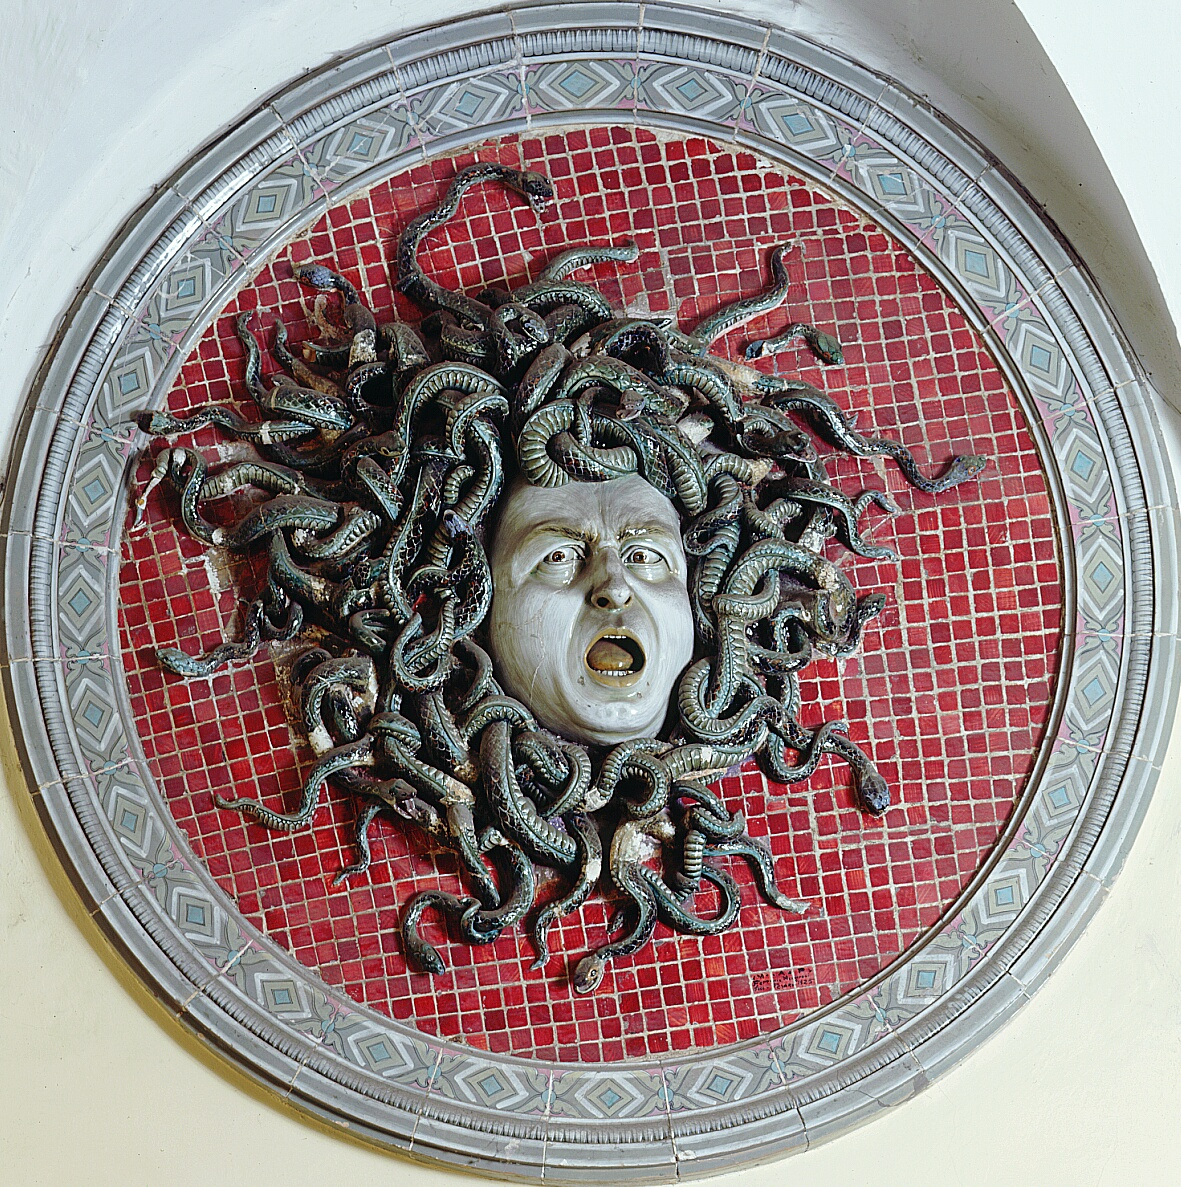
\includegraphics[]{Mengaroni_Ferruccio-Medusa.jpg}
				\captionof{figure}{Mengaroni Ferruccio - Medusa.}
			\end{minipage}
		\end{itemize}
	\end{frame}
	
	\begin{frame}{\numcirc{2} Mostrare la Pala Bellini.}
		\begin{itemize}
			\item Mostrare la \textbf{Pala Bellini} (presente nella sala Bellini). Evidenziando il dettaglio della \textit{Colomba} che rappresenta lo \textit{Spirito Santo}, presente nel pannello centrale contenente la scena dell'Incoronazione della Vergine e il dettaglio del \textit{Drago di S. Giorgio e il Drago}, presente in basso tra i sette riquadri della predella.\par
		\end{itemize}
	\end{frame}

	\begin{frame}
		\bigskip
			\begin{minipage}{\linewidth}
			\centering
			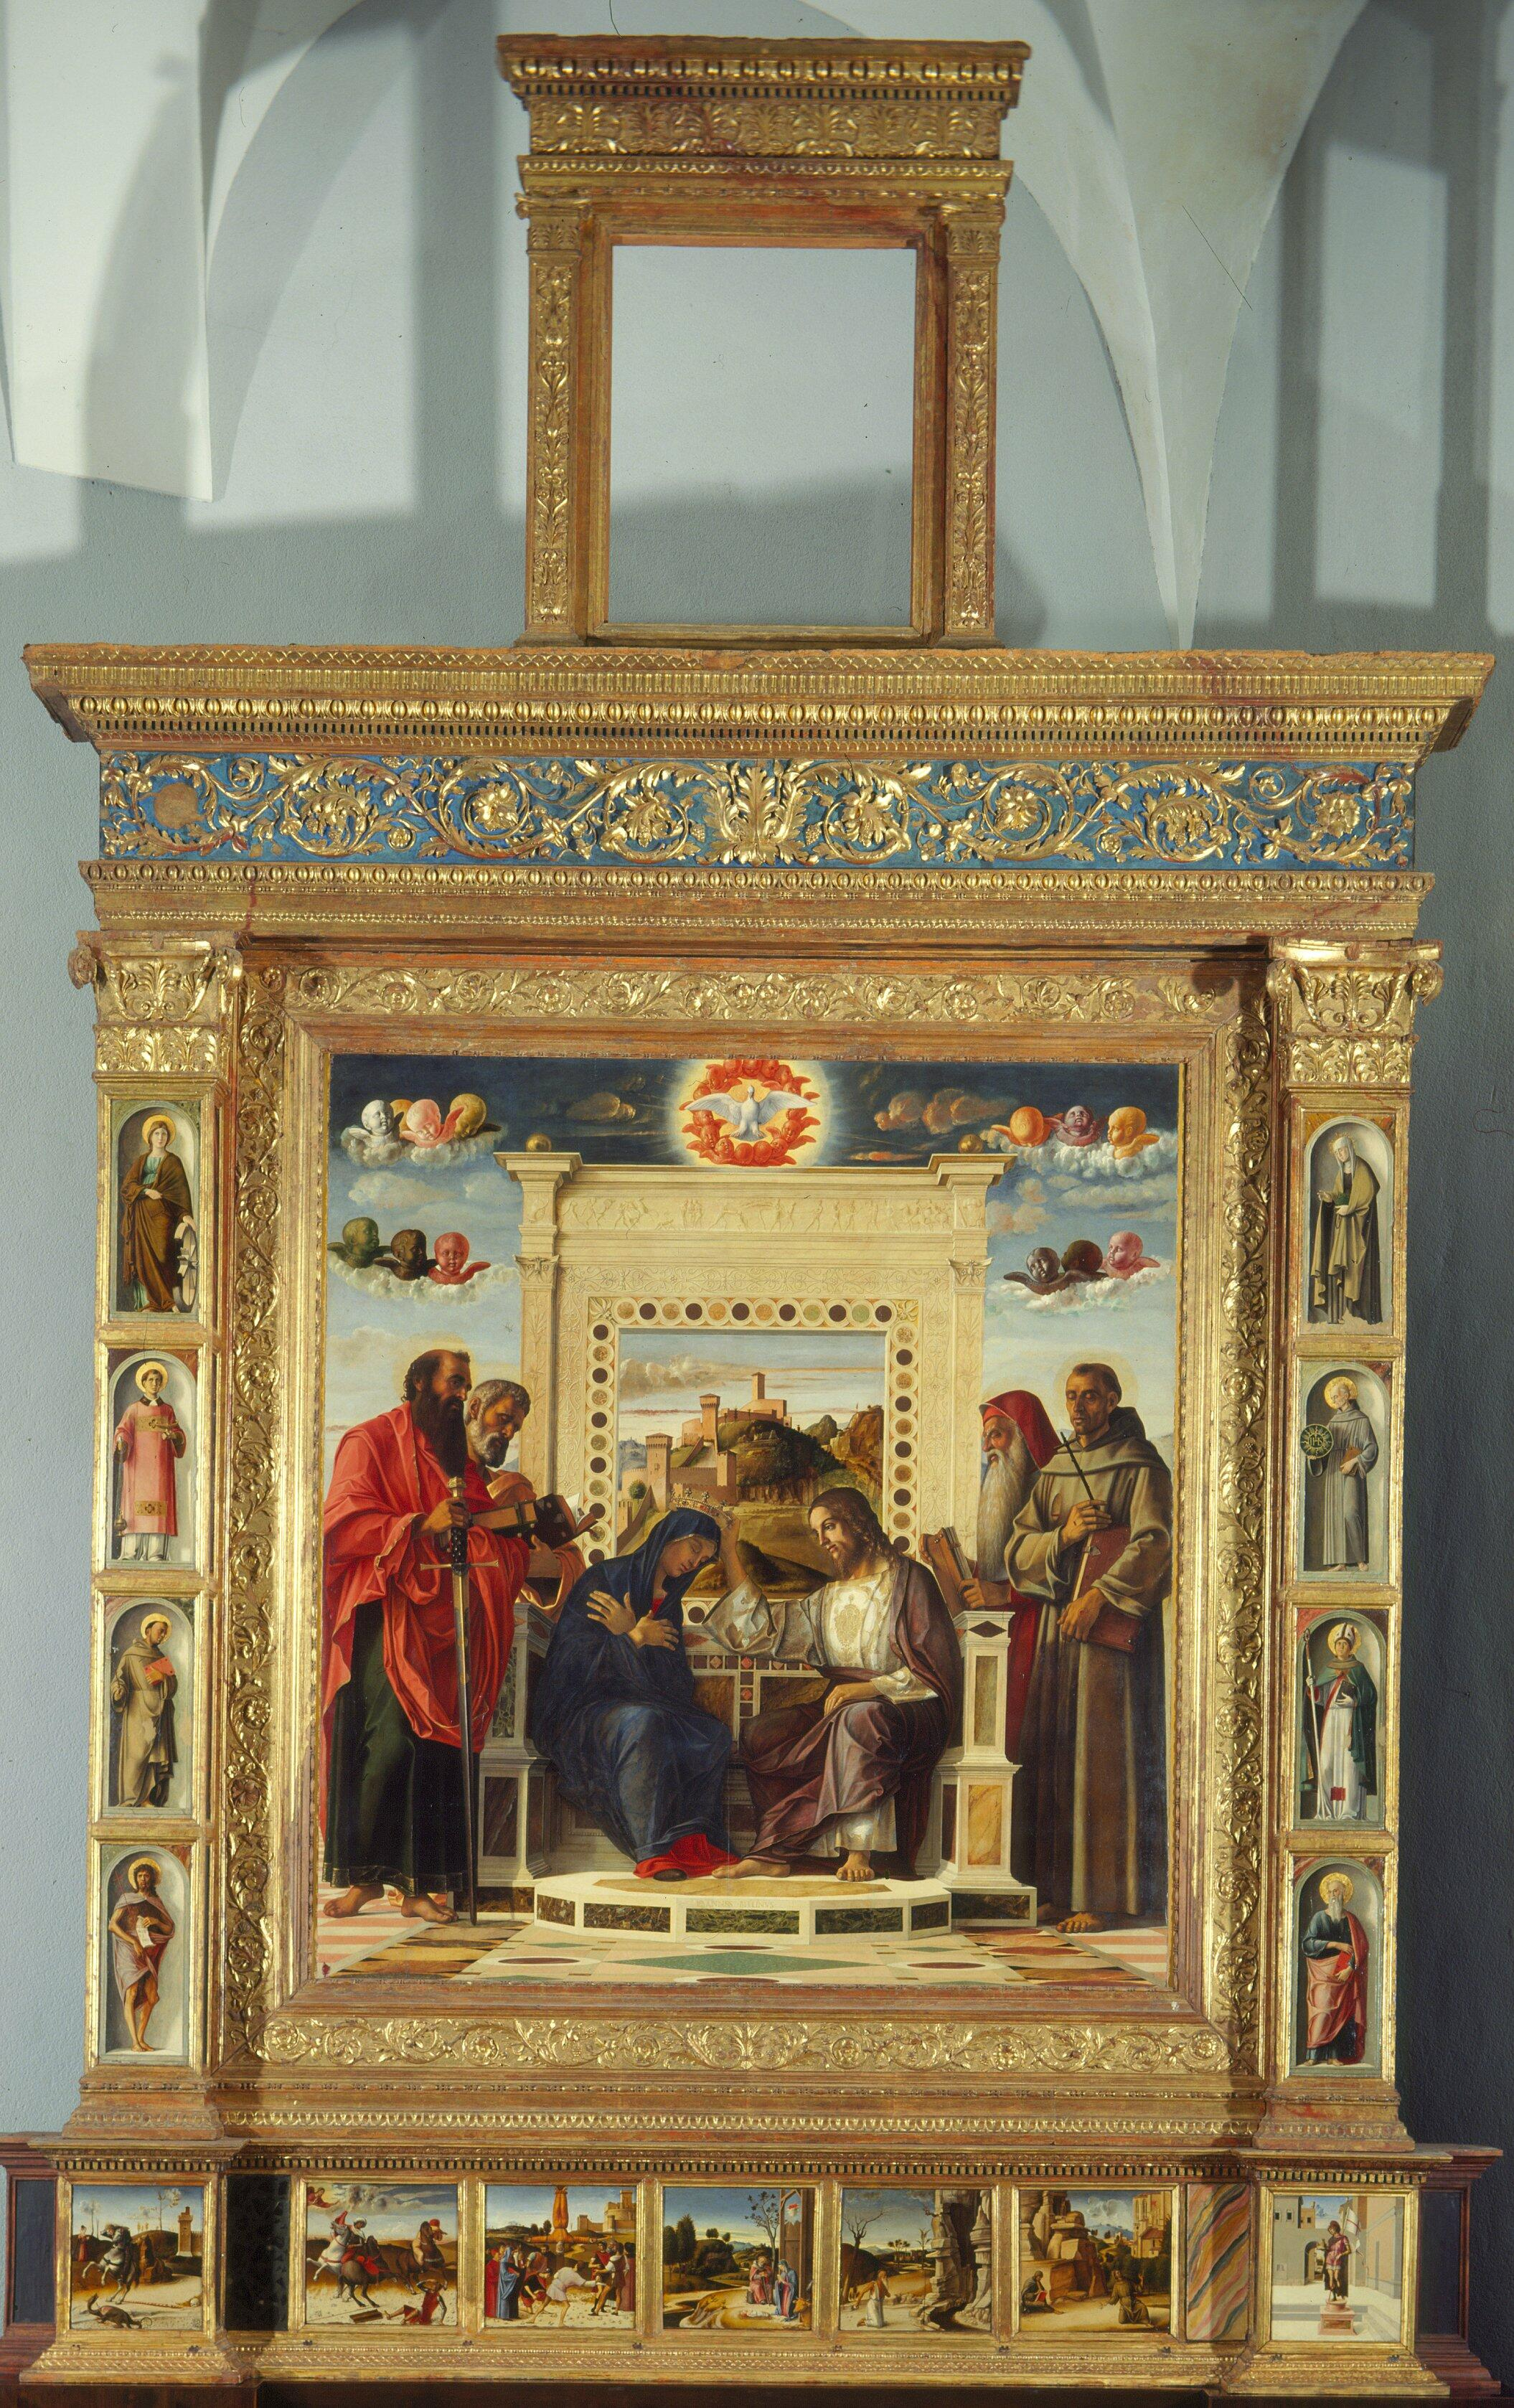
\includegraphics[scale=0.063]{Bellini_Giovanni-Incoronazione_della_Vergine.jpg}
			\captionof{figure}{Bellini Giovanni - Incoronazione della Vergine.}
		\end{minipage}
	\end{frame}

	\begin{frame}
		\begin{minipage}{\linewidth}
			\centering
			\begin{minipage}{0.4\linewidth}
				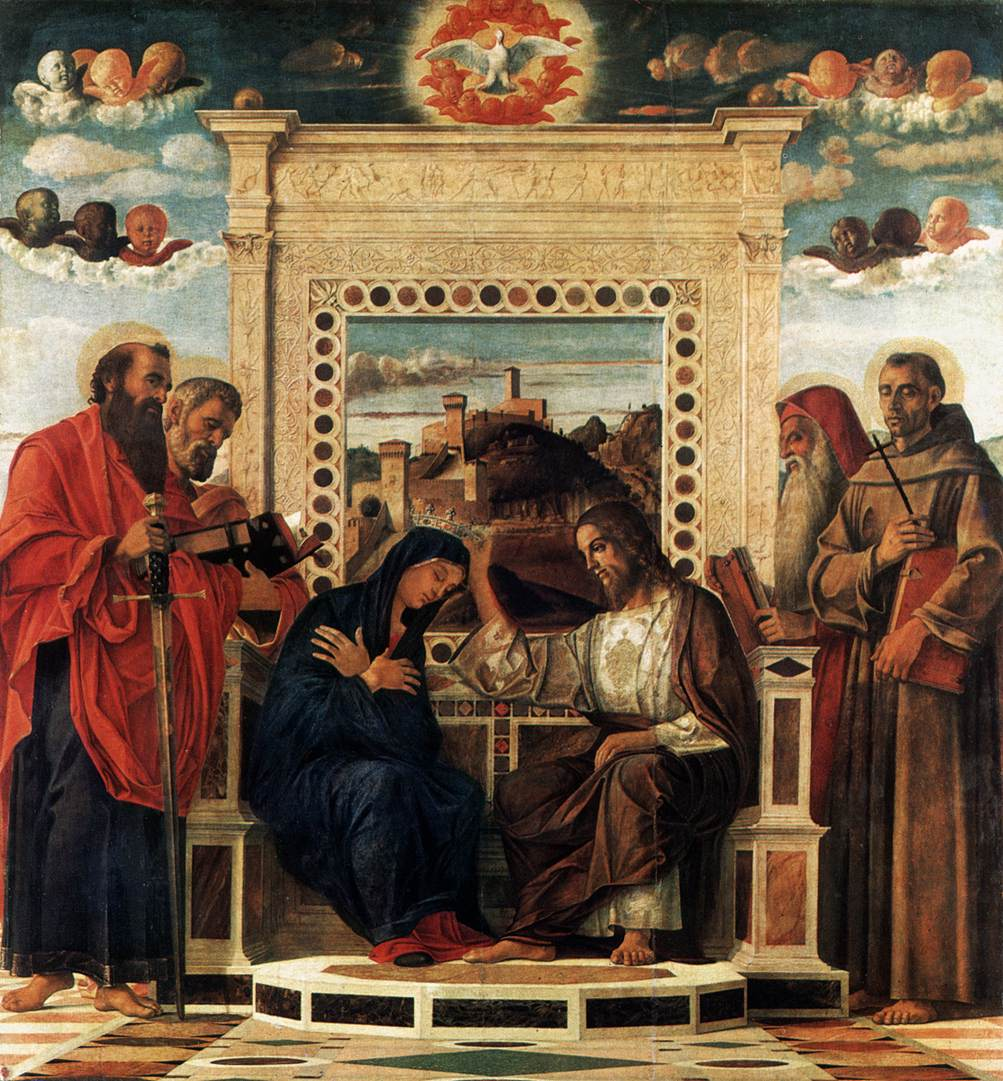
\includegraphics[scale=0.65]{Pala_di_pesaro_incoronazione.jpg}
				\captionof{figure}{Dettaglio: Incoronazione della Vergine.}
			\end{minipage}
			\hfill
			\begin{minipage}{0.4\linewidth}
				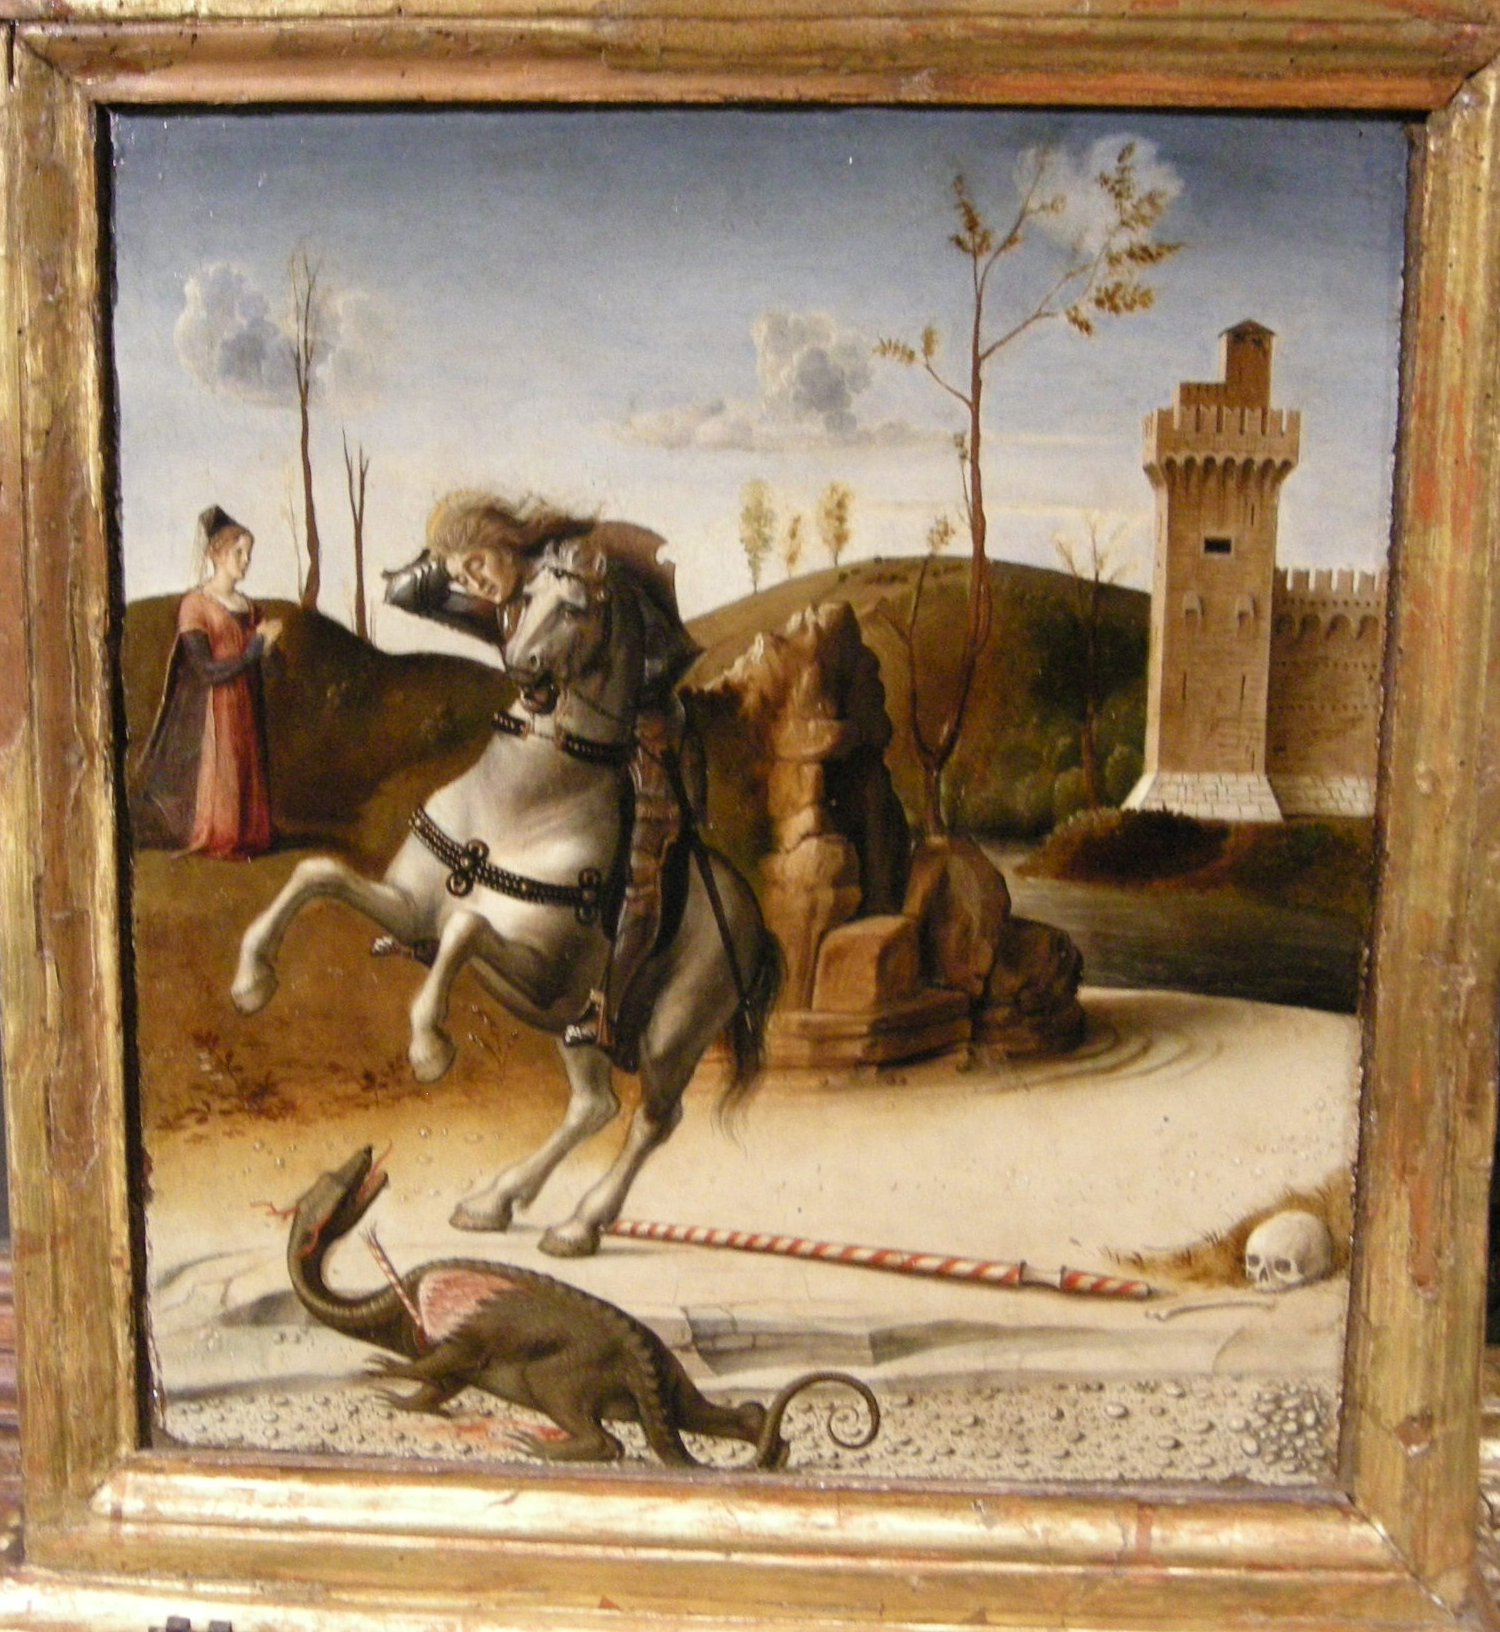
\includegraphics[scale=0.1]{Pala_di_Pesaro_S.Giorgio_e_il_Drago.jpg}
				\captionof{figure}{Dettaglio: S. Giorgio e il Drago.}
			\end{minipage}
		\end{minipage}
	\end{frame}

	\begin{frame}{\numcirc{3} Mostrare quadri che fanno più o meno uso della prospettiva.}
		\begin{itemize}
			\item Mostrare quadri che fanno uso della prospettiva, confrontandoli con quelli che ne sono privi. \par 
		\end{itemize}
	\end{frame}

	\begin{frame}
		\bigskip
		\begin{minipage}{\linewidth}
			\centering
			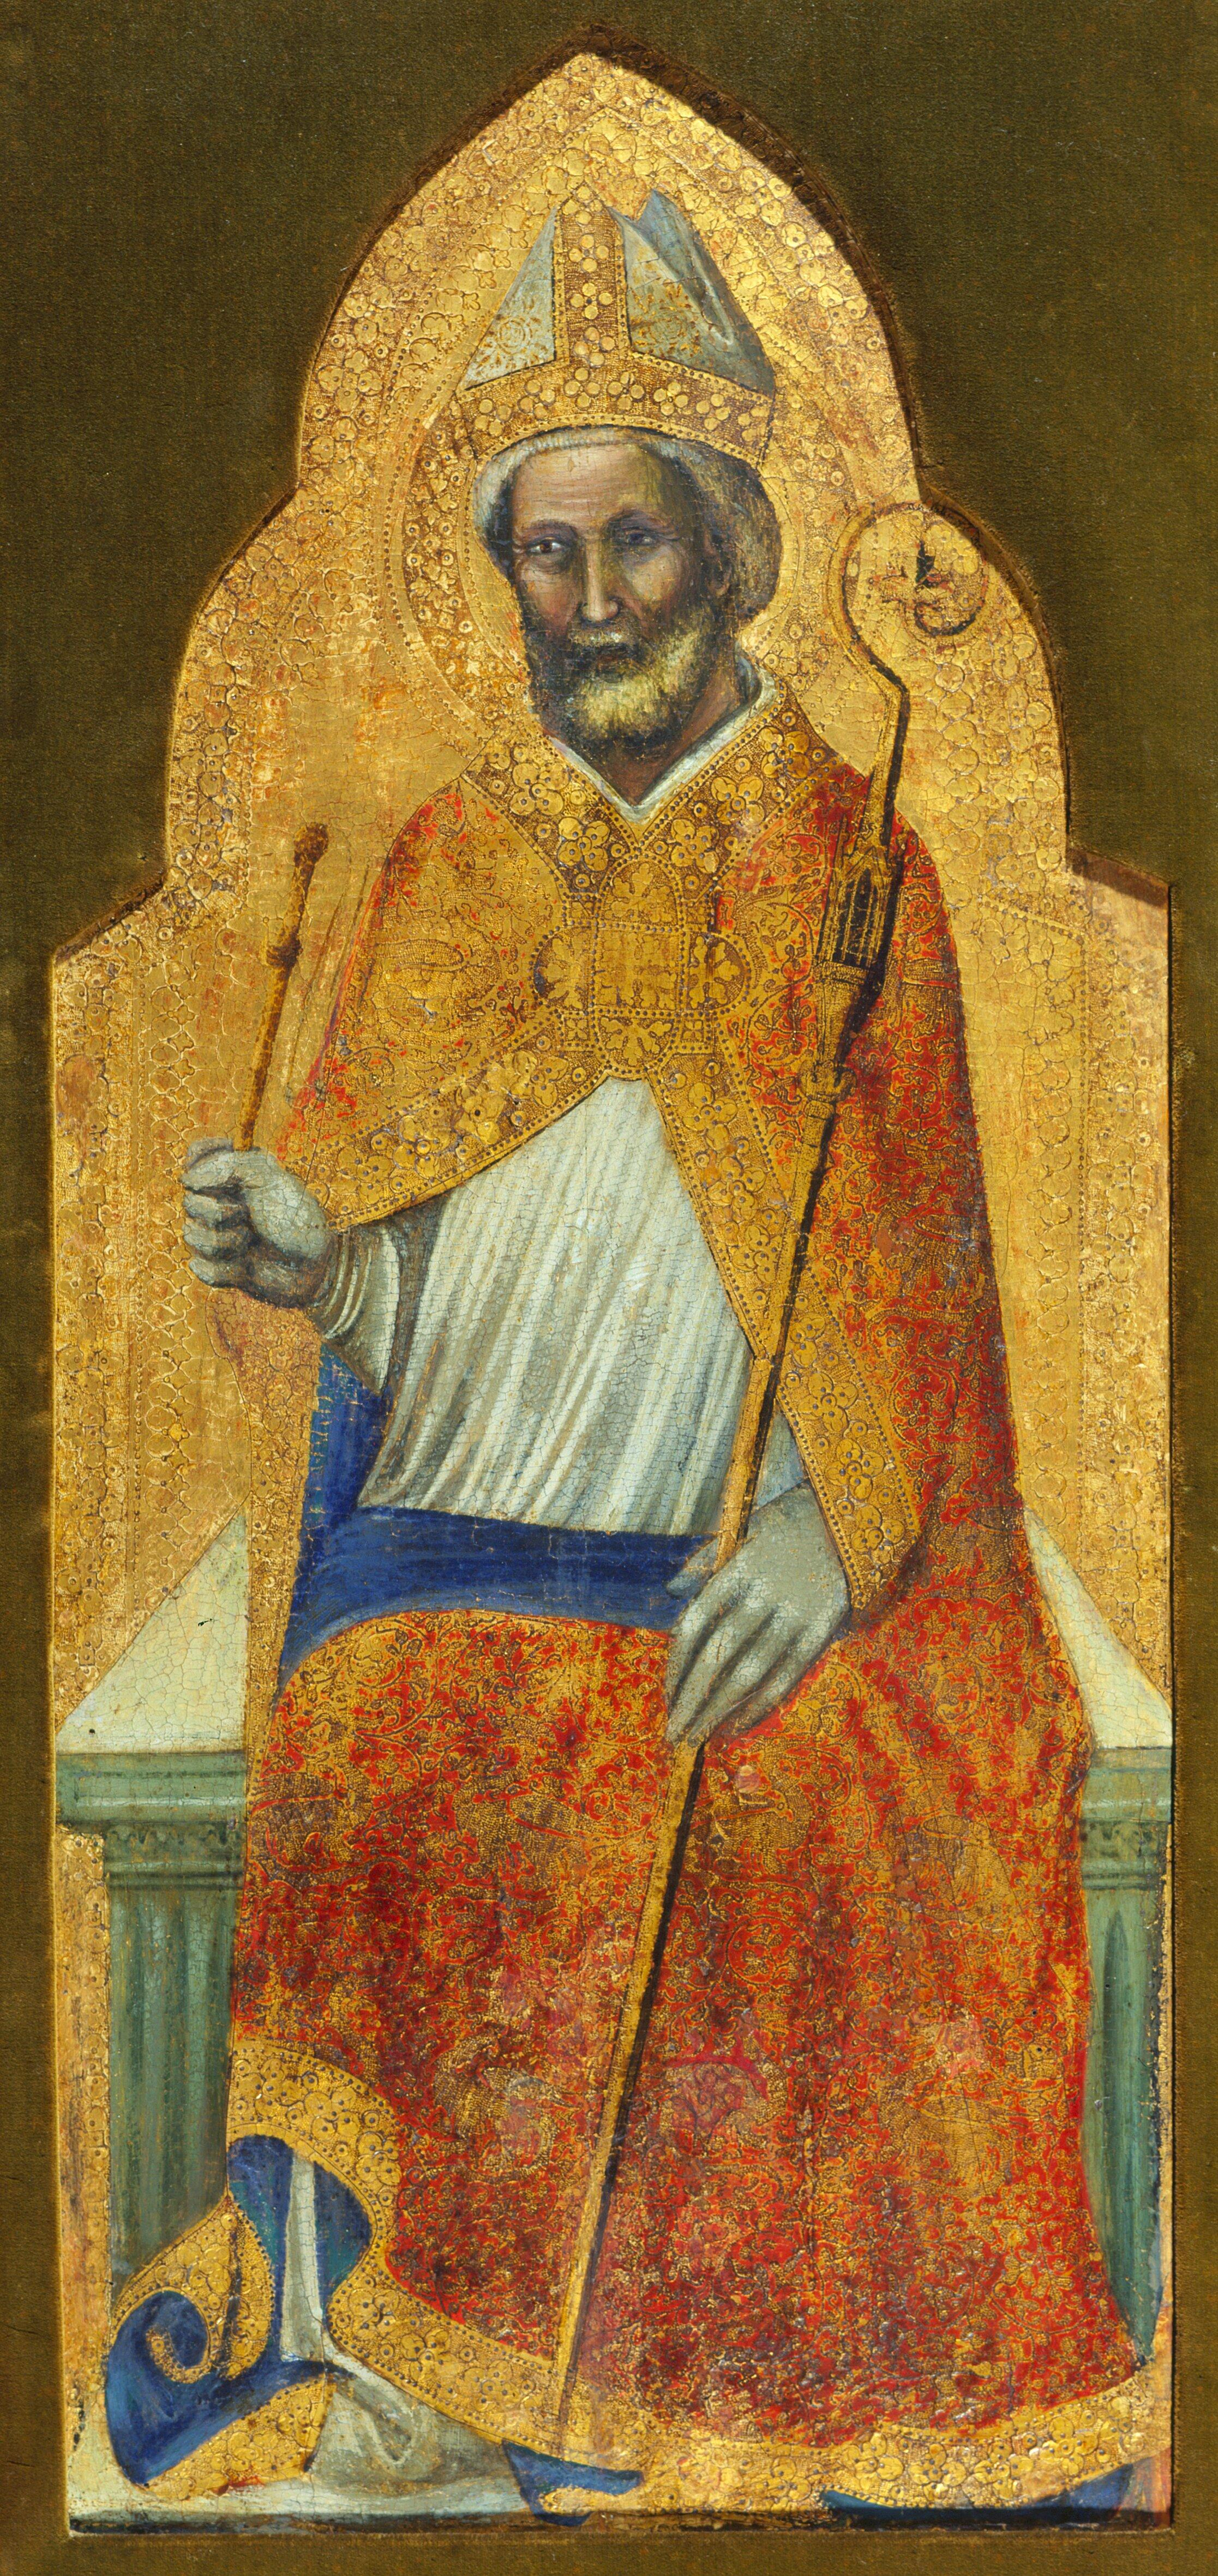
\includegraphics[scale=0.043]{Vitale_da_Bologna-Santo_Ambrogio_in_trono.jpg}
			\captionof{figure}{Vitale da Bologna - Santo Ambrogio in trono. \\ \centering Esempio di quadro senza prospettiva.}
		\end{minipage} 
	\end{frame}

	\begin{frame}{\numcirc{4} Spiegare gli elementi che contraddistinguono la Collezione Rossini.}
		\begin{itemize}
			\item Spiegare gli elementi che contraddistinguono la \textbf{Collezione Rossini}; come il \textit{Rosso vermiglio} e \textit{l'oro ed i gioielli} nei dipinti.\par \bigskip
			\begin{minipage}{\linewidth}
				\centering
				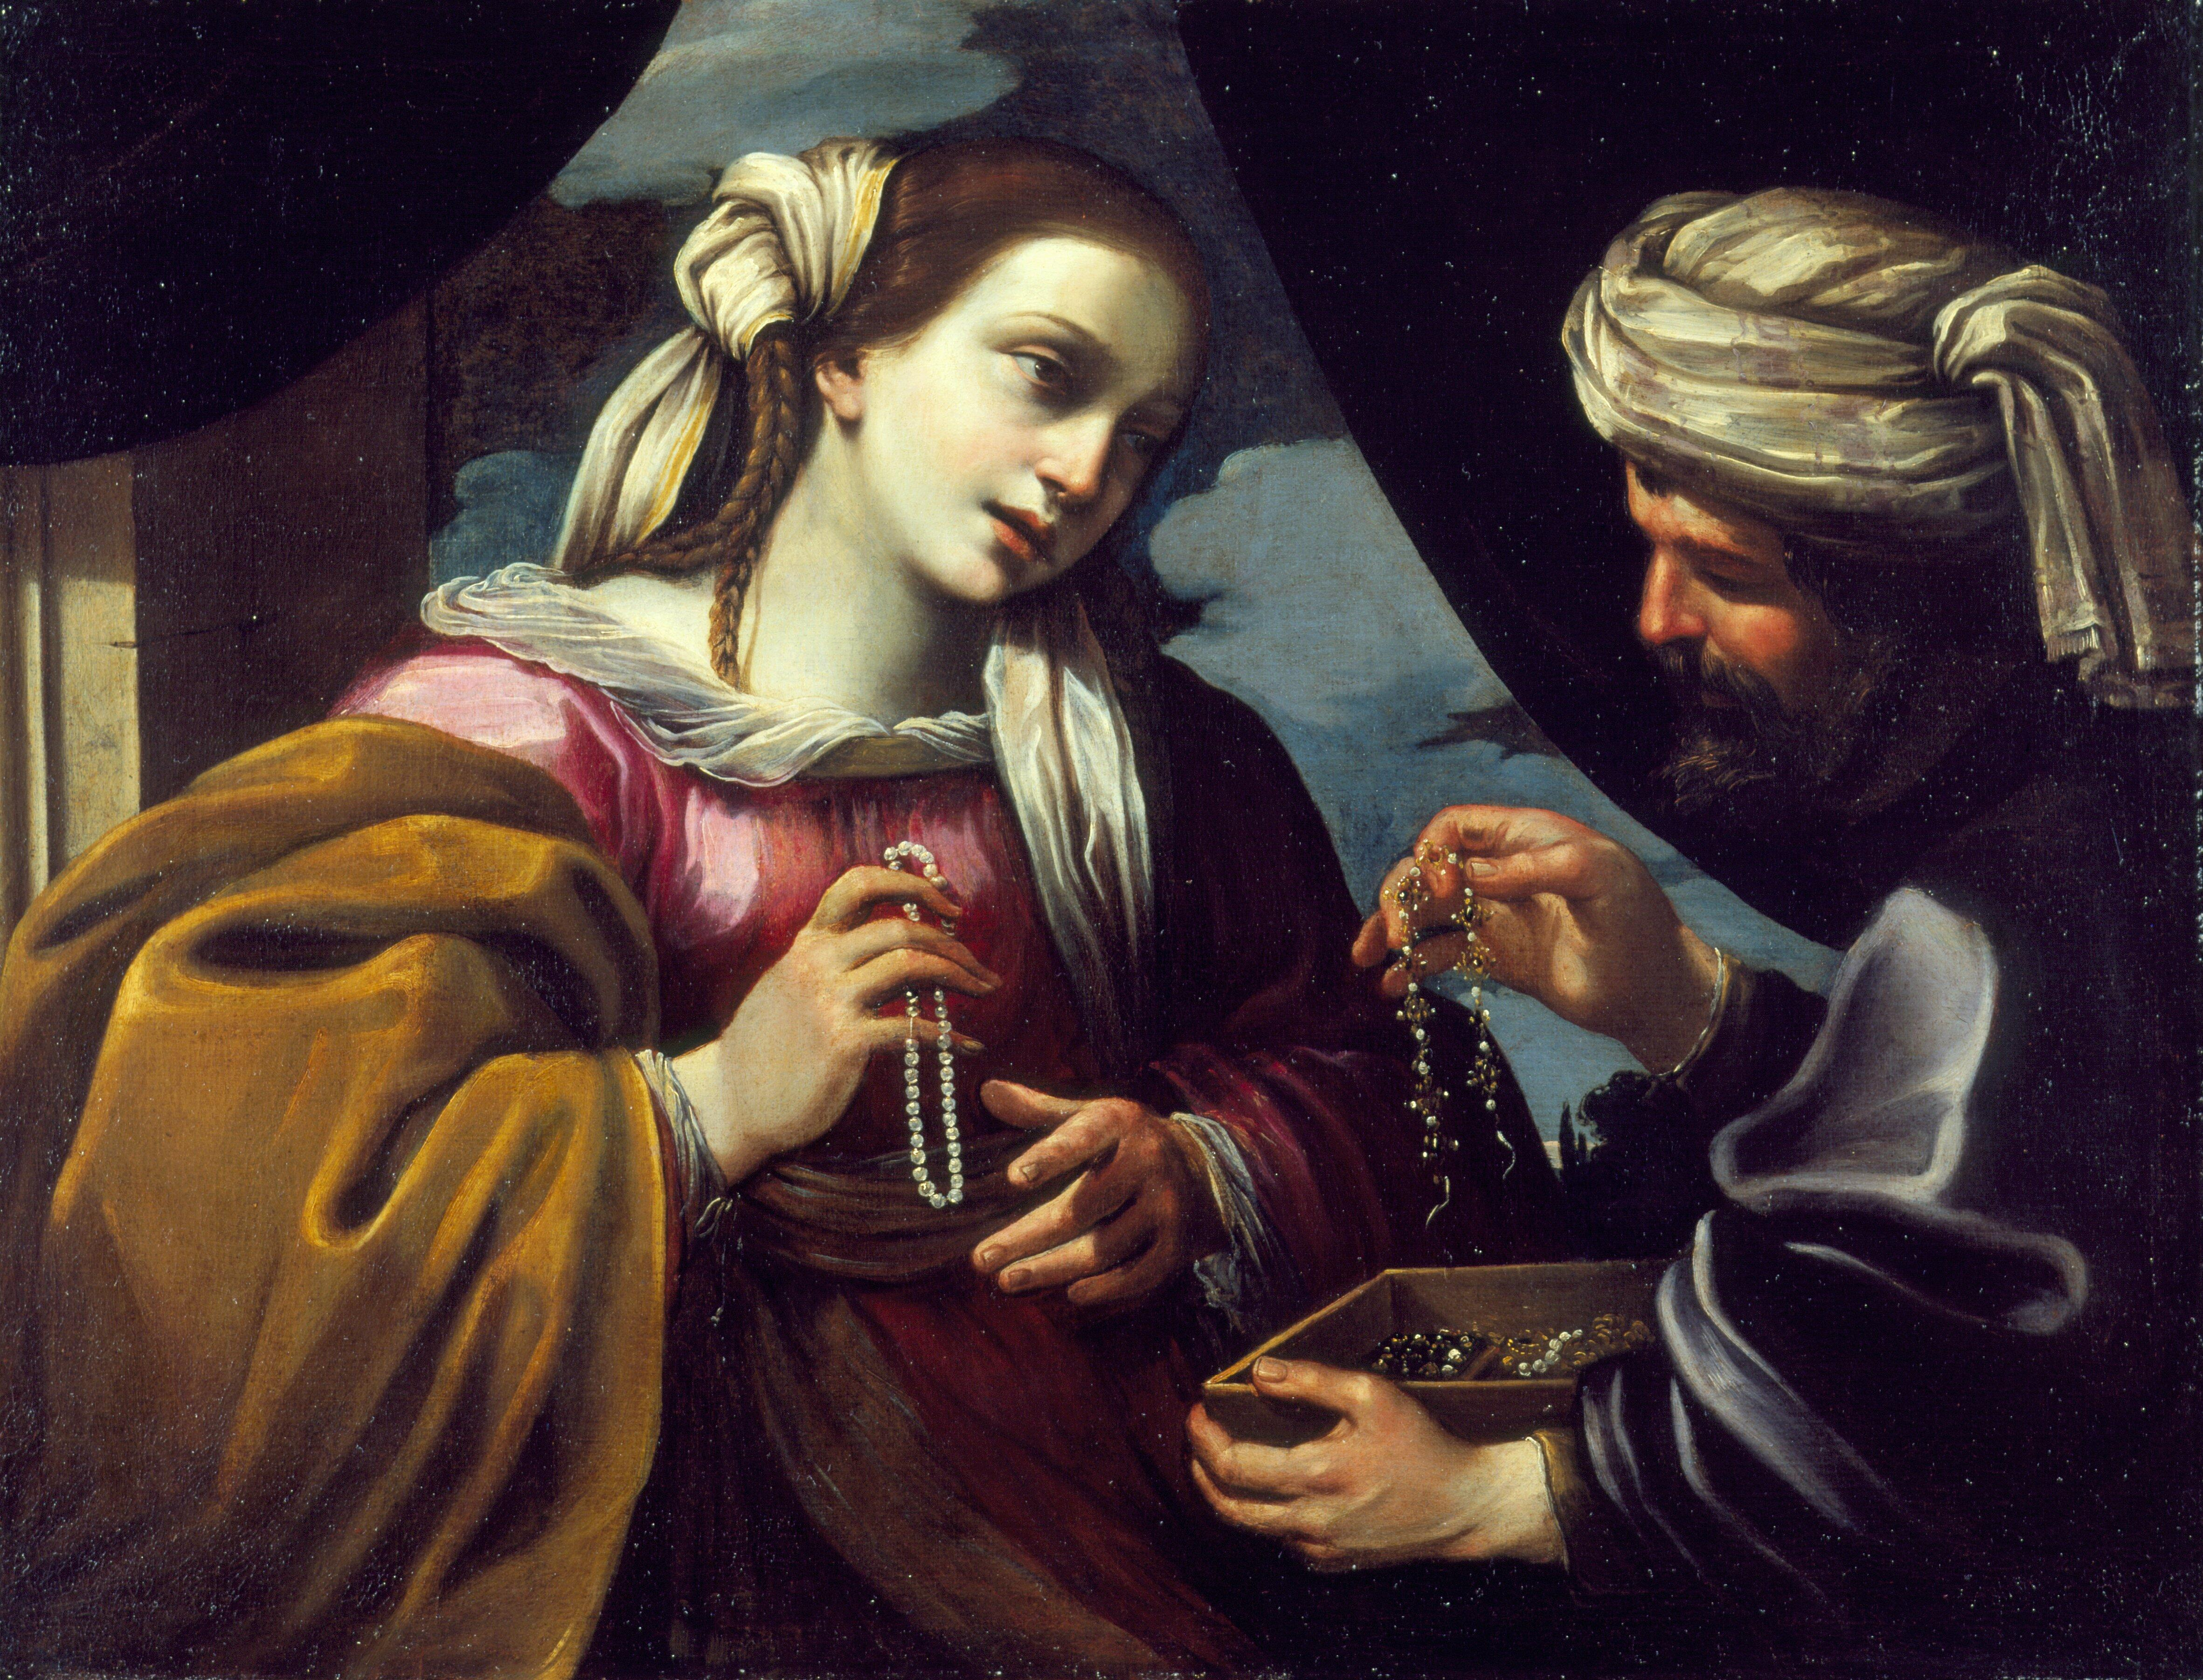
\includegraphics[scale = 0.042]{Desani_Pietro-Rebecca_ed_Eleazar.jpg}
				\captionof{figure}{Desani Pietro - Rebecca ed Eleazar.}
			\end{minipage}
		\end{itemize}
	\end{frame}

	\begin{frame}{\numcirc{5} Mostrare il piatto dove è presente lo scoiattolo nero.}
		\begin{itemize}
			\item Mostrare la \textbf{ceramica della collezione Mazza} dove è presente lo \textit{scoiattolo nero di cinquecento anni fa}.\par \bigskip
			\begin{minipage}{\linewidth}
				\centering
				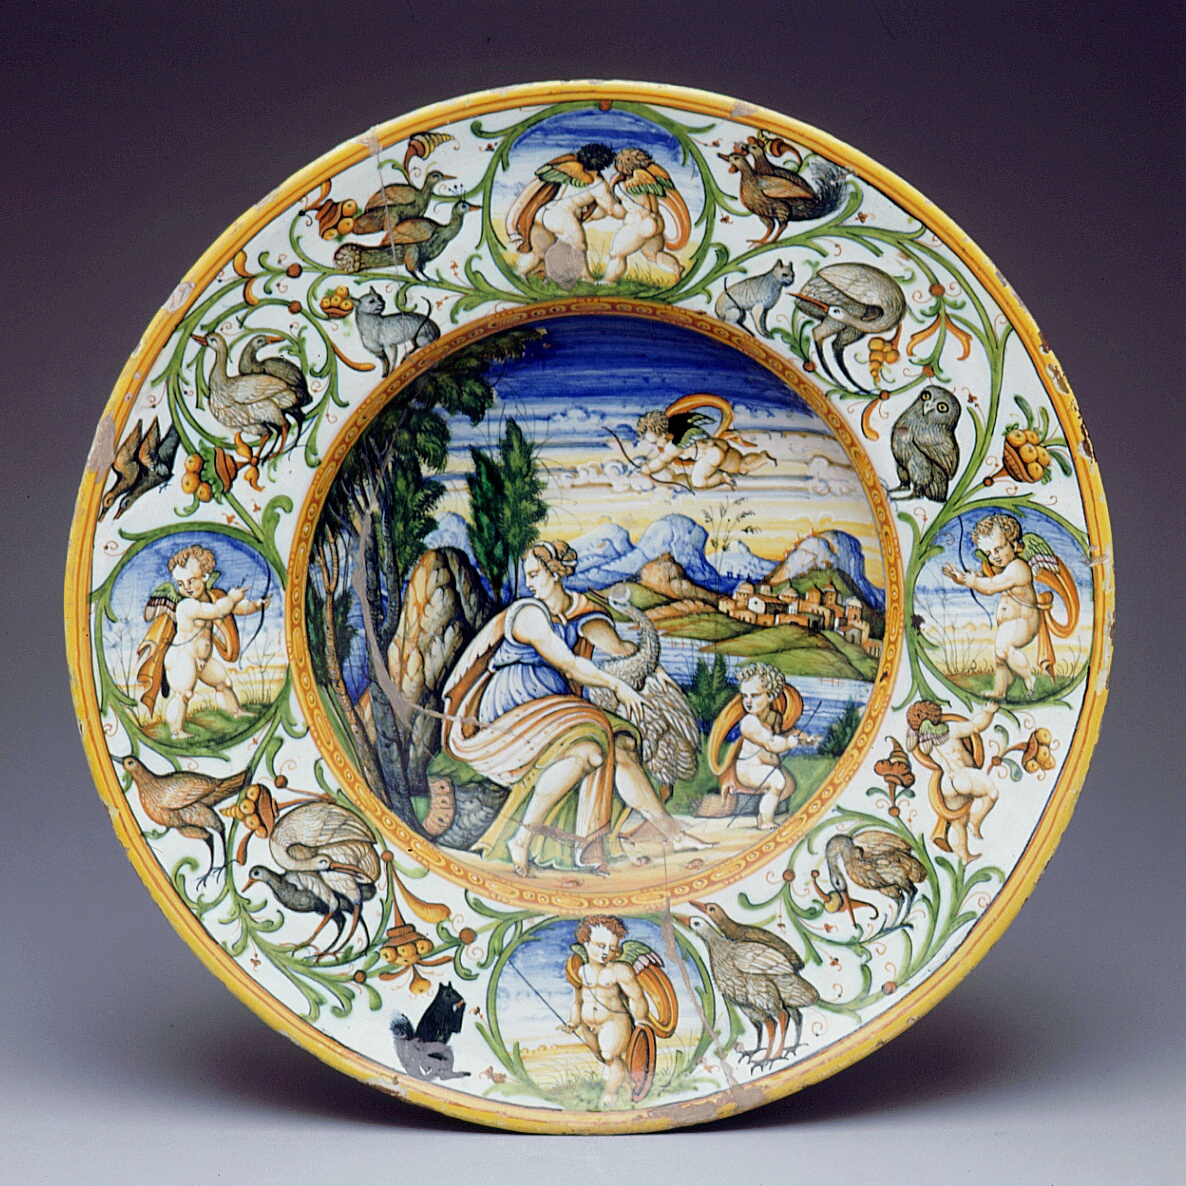
\includegraphics[]{Pittore_della_Conversione_di_San_Paolo-Leda_e_il_cigno.jpg}
				\captionof{figure}{Leda e il Cigno (Giove) di fattura ad opera di Giovanni Antonio Garella.}
			\end{minipage}
		\end{itemize}
	\end{frame}
	
	\begin{frame}{\numcirc{6} Esporre: lo specchio in vetro di Murano, gli oggetti in avorio e madreperla, lo stipo con vedute di Roma e l'orologio notturno.}
		\begin{itemize}
			\item Esporre in maniera semplice: lo \textbf{specchio in vetro di Murano} decorato con \textit{incisioni d'uva d'argento},  gli \textbf{oggetti in avorio e madreperla}, lo \textbf{Stipo con vedute di Roma} facendo riferimento alle \textit{cartoline} di Roma e l'\textbf{Orologio Notturno}.\par
		\end{itemize}
	\end{frame}

	\begin{frame}
		\bigskip
		\begin{minipage}{\linewidth}
			\centering
			\begin{minipage}{0.4\linewidth}
				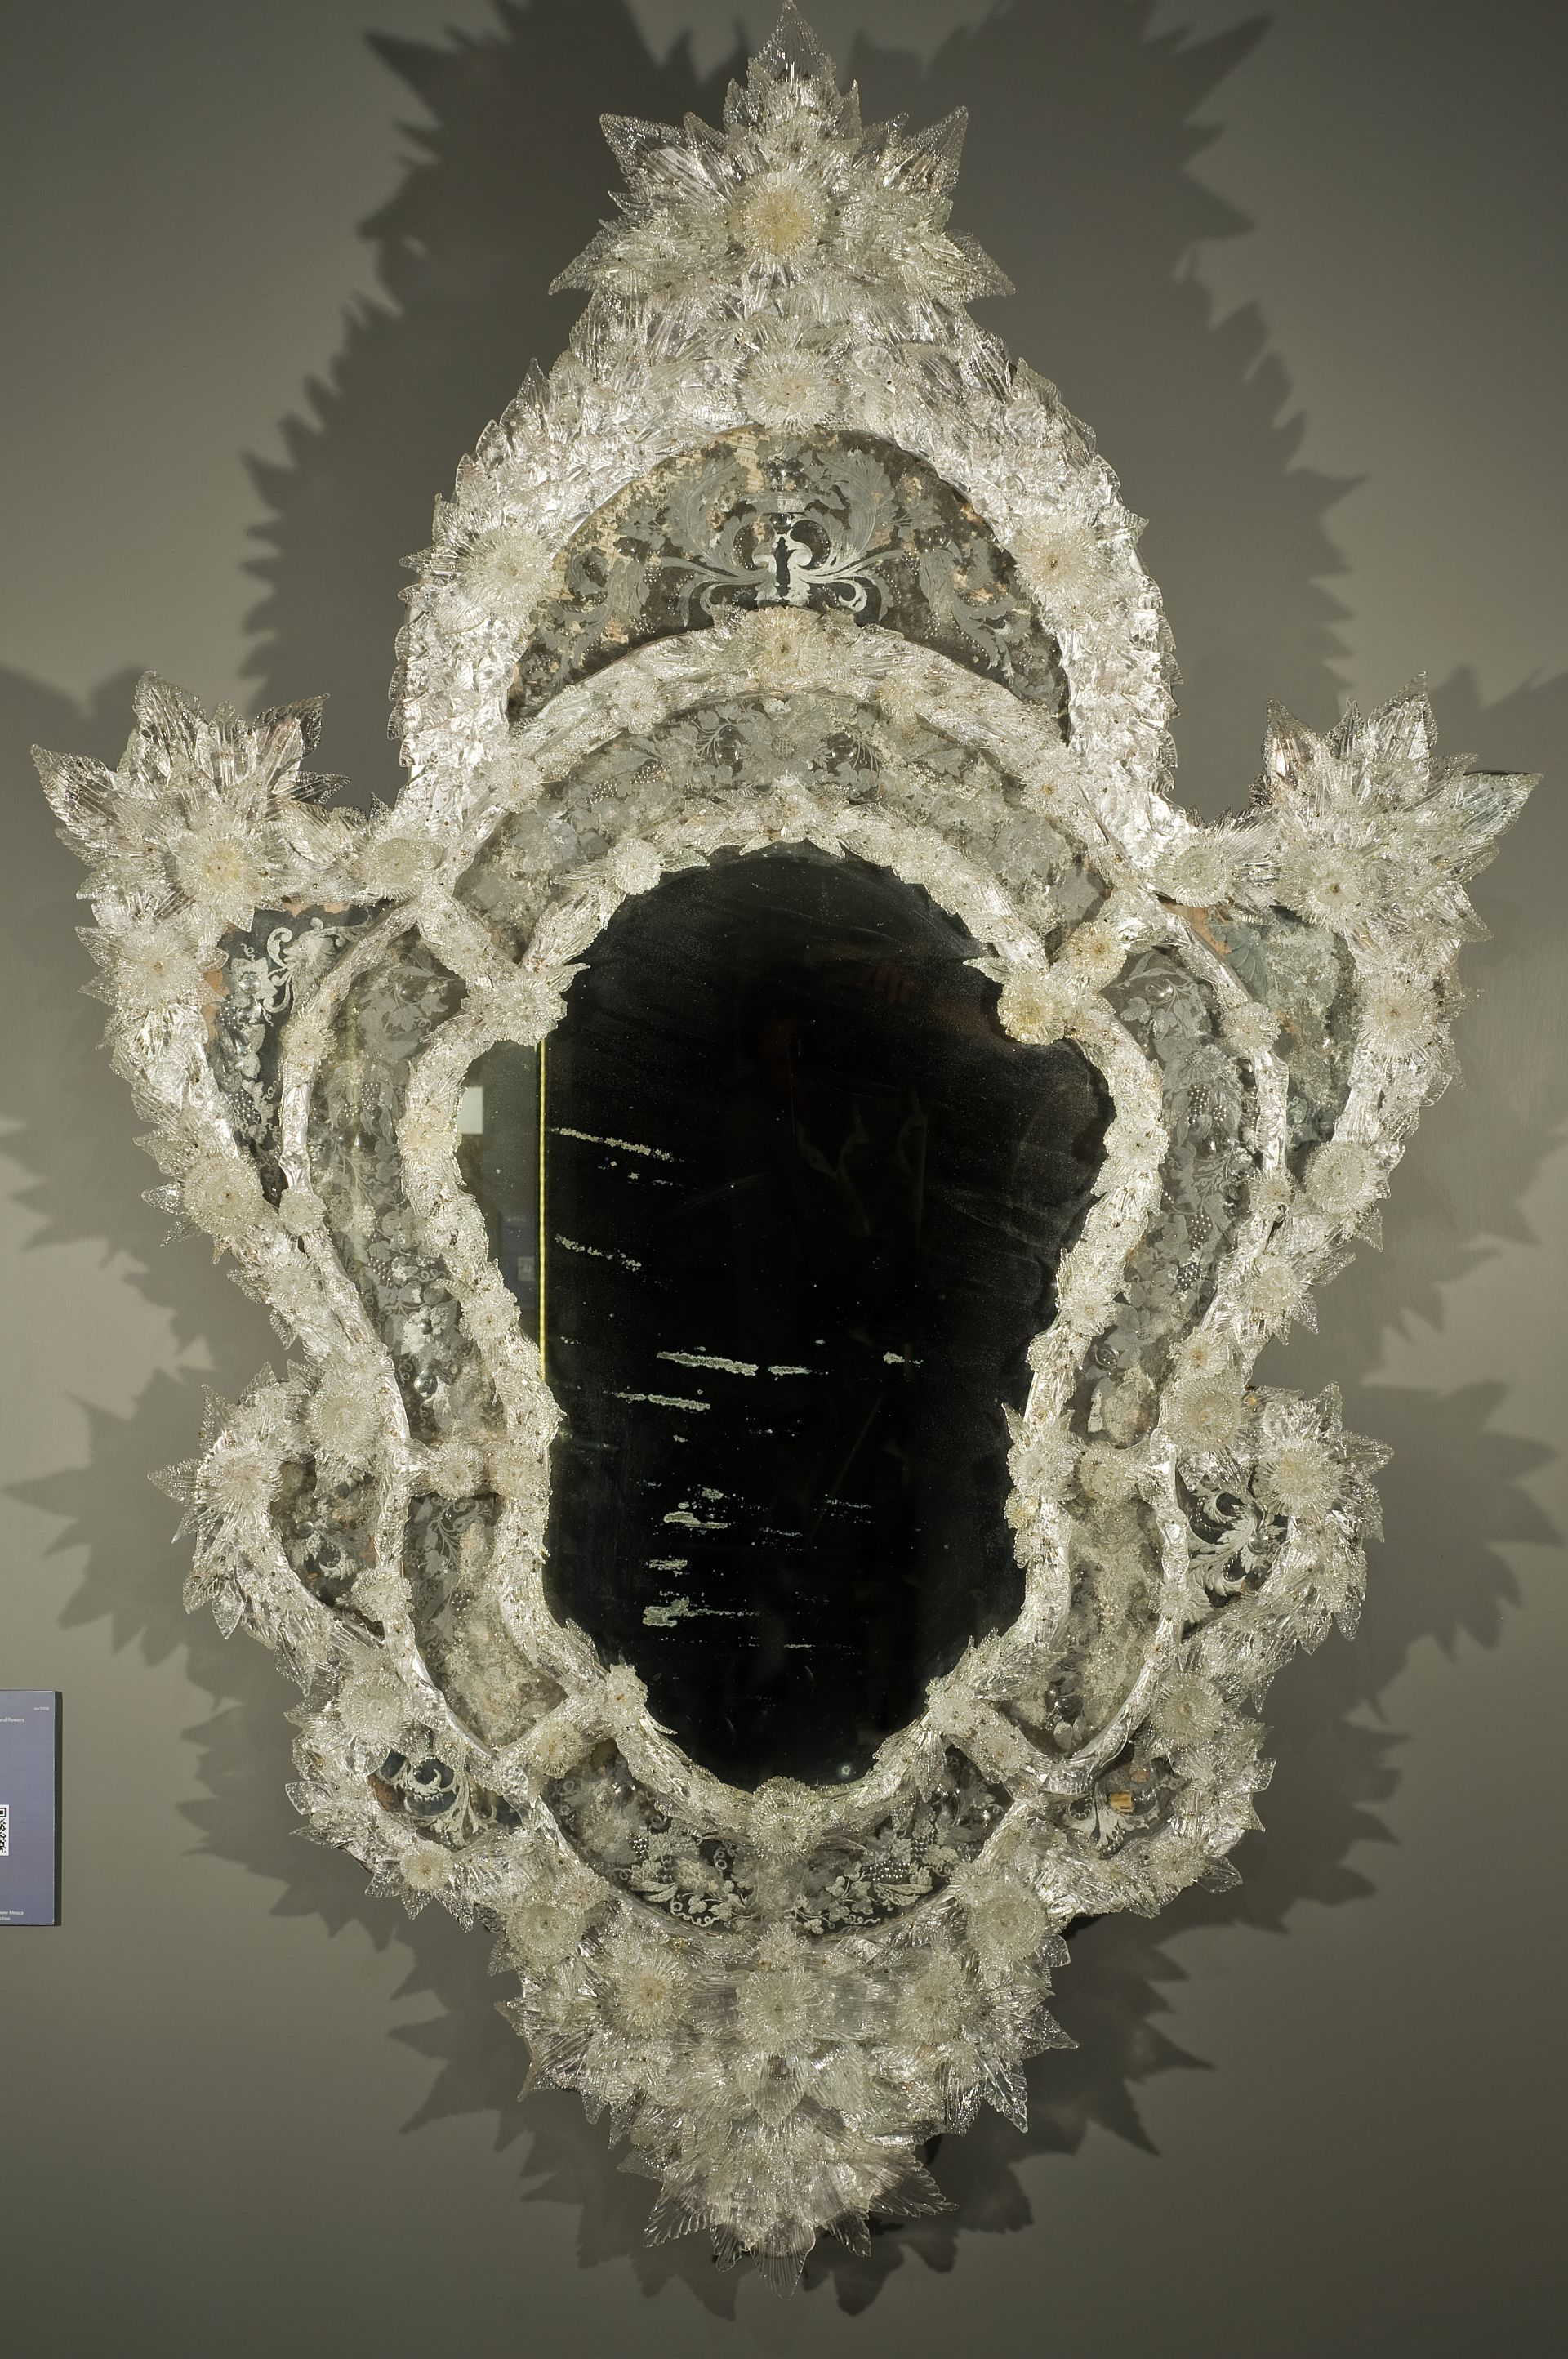
\includegraphics[scale=0.23]{Specchio_di_Murano.jpg}
				\captionof{figure}{Specchio in vetro di Murano.}
			\end{minipage}
			\hfill
			\begin{minipage}{0.4\linewidth}
				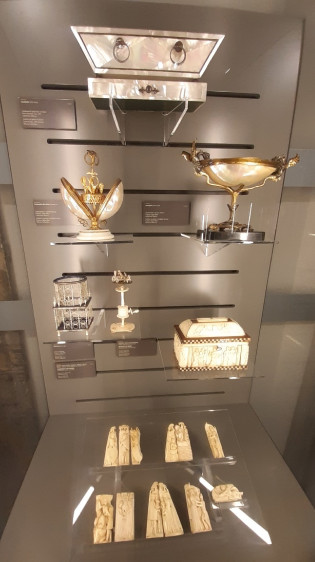
\includegraphics[scale=1.45]{Avorio_madreperla.jpg}
				\captionof{figure}{Oggetti in avorio e madreperla.}
			\end{minipage}
		\end{minipage}
	\end{frame}

	\begin{frame}
		\bigskip
		\begin{minipage}{\linewidth}
			\centering
			\begin{minipage}{0.4\linewidth}
				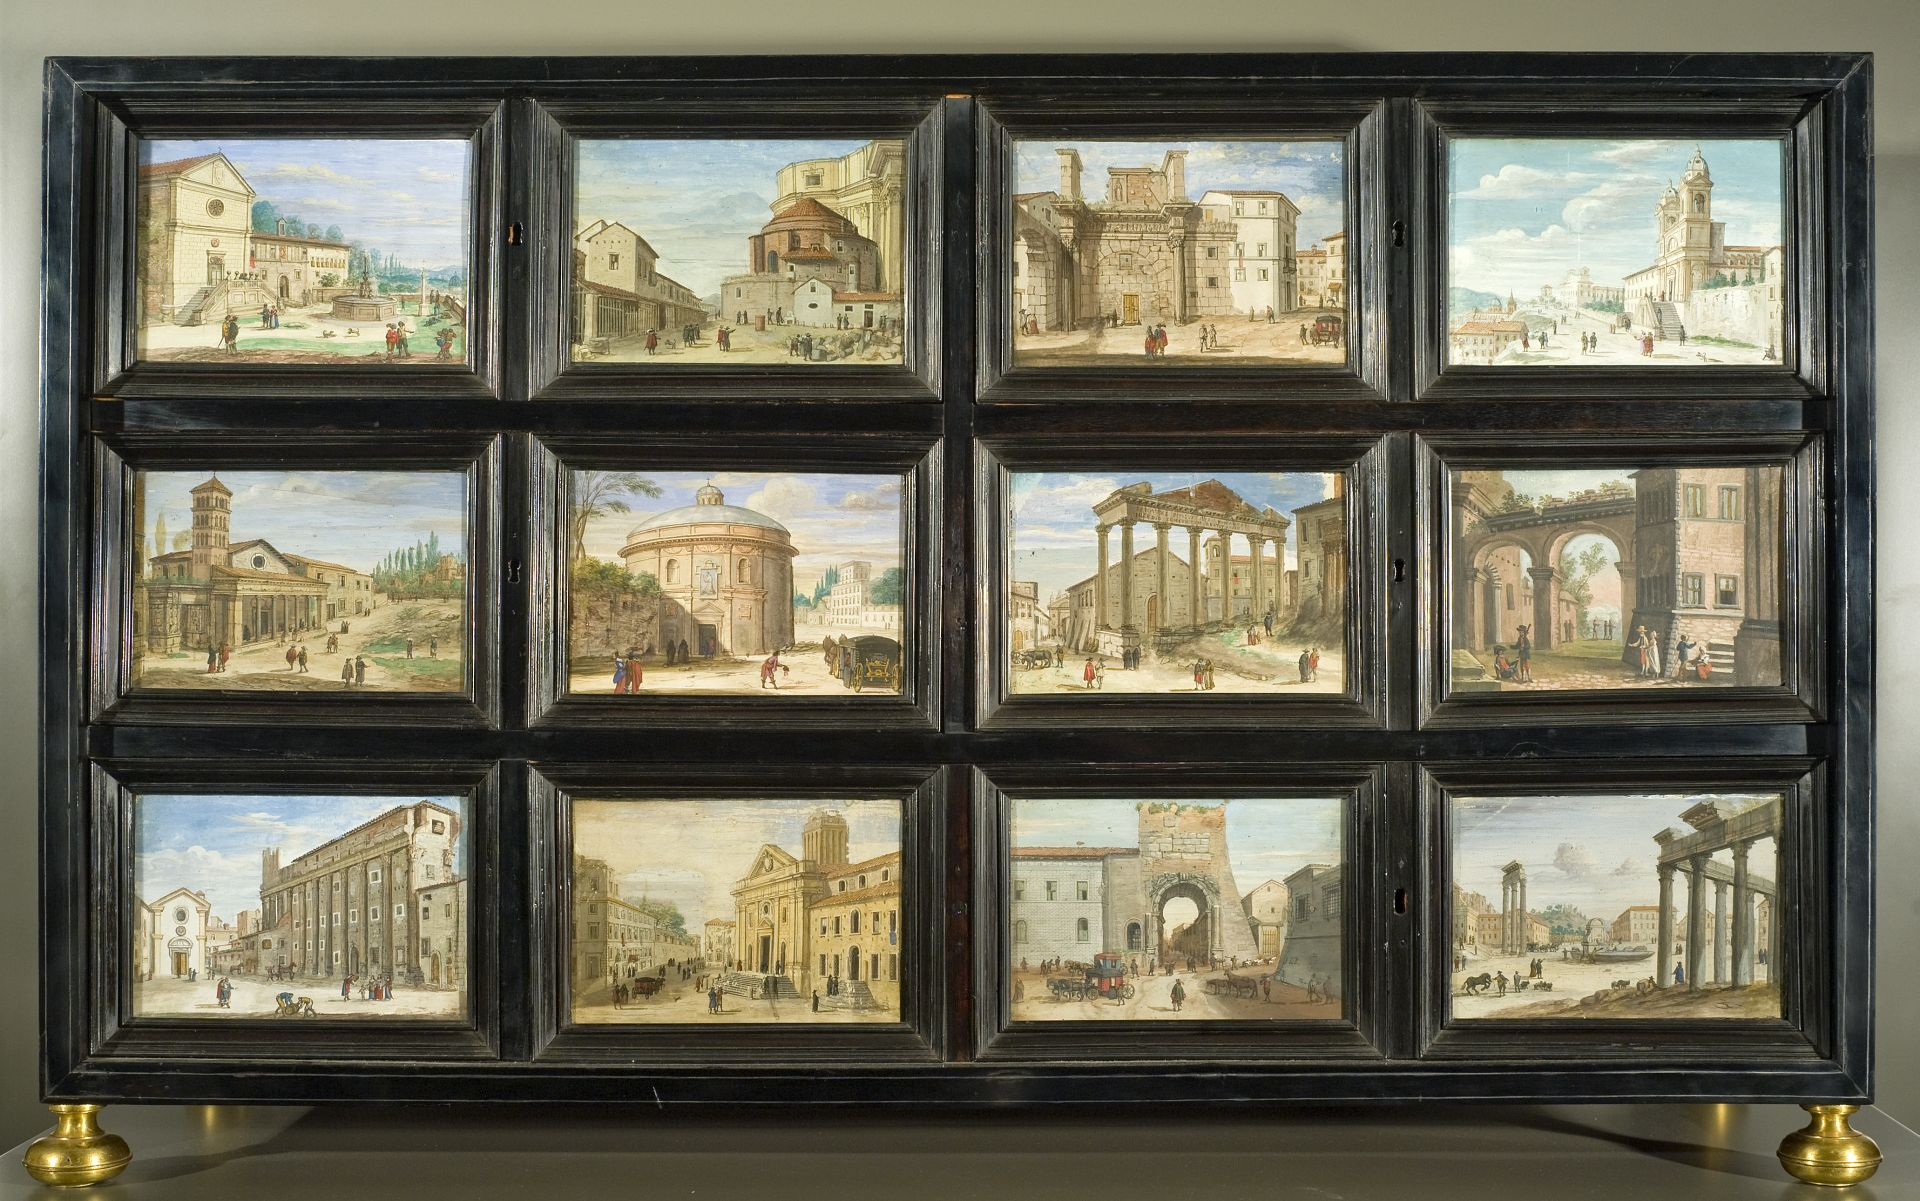
\includegraphics[scale=0.4]{Vedute_di_Roma_1.jpg}
				\captionof{figure}{Vedute di Roma.}
			\end{minipage}
			\hfill
			\begin{minipage}{0.4\linewidth}
				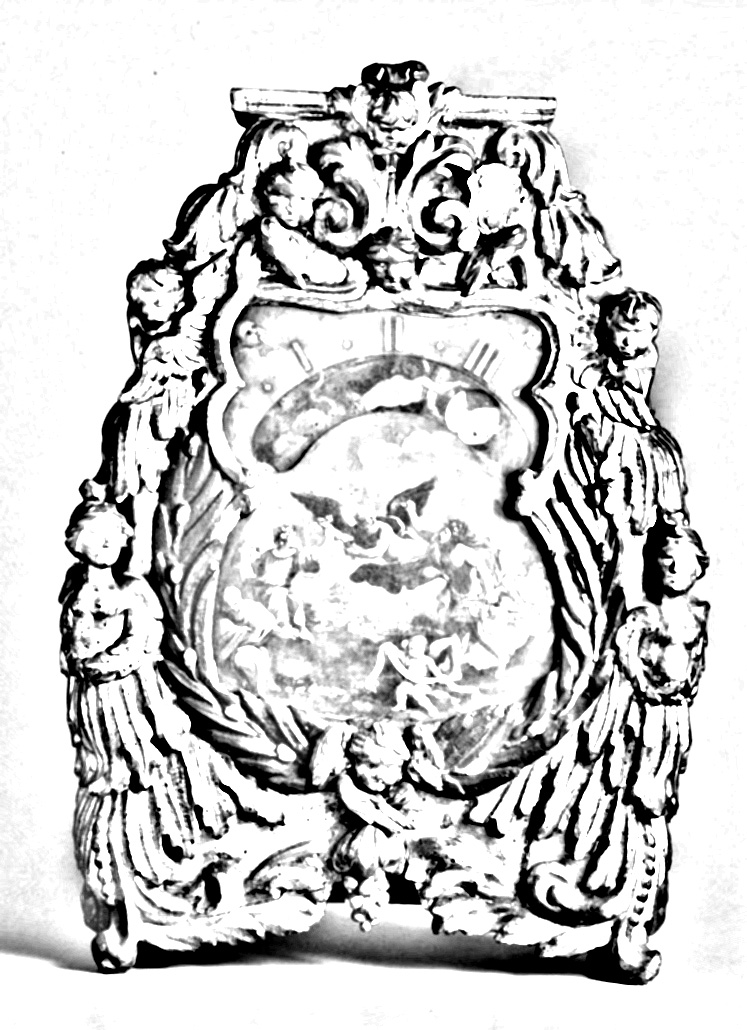
\includegraphics[scale=0.2]{Orologio_notturno.jpg}
				\captionof{figure}{Orologio notturno.}
			\end{minipage}
		\end{minipage}
	\end{frame}
	
	\begin{frame}{\numcirc{7} Mostrare il piatto decorato con la Rosa di Pesaro.}
		\begin{itemize}
			\item Mostrare il \textbf{Piatto della bottega pesarese} con \textit{decoro della Rosa di Pesaro}.\par \bigskip
			\begin{minipage}{\linewidth}
				\centering
				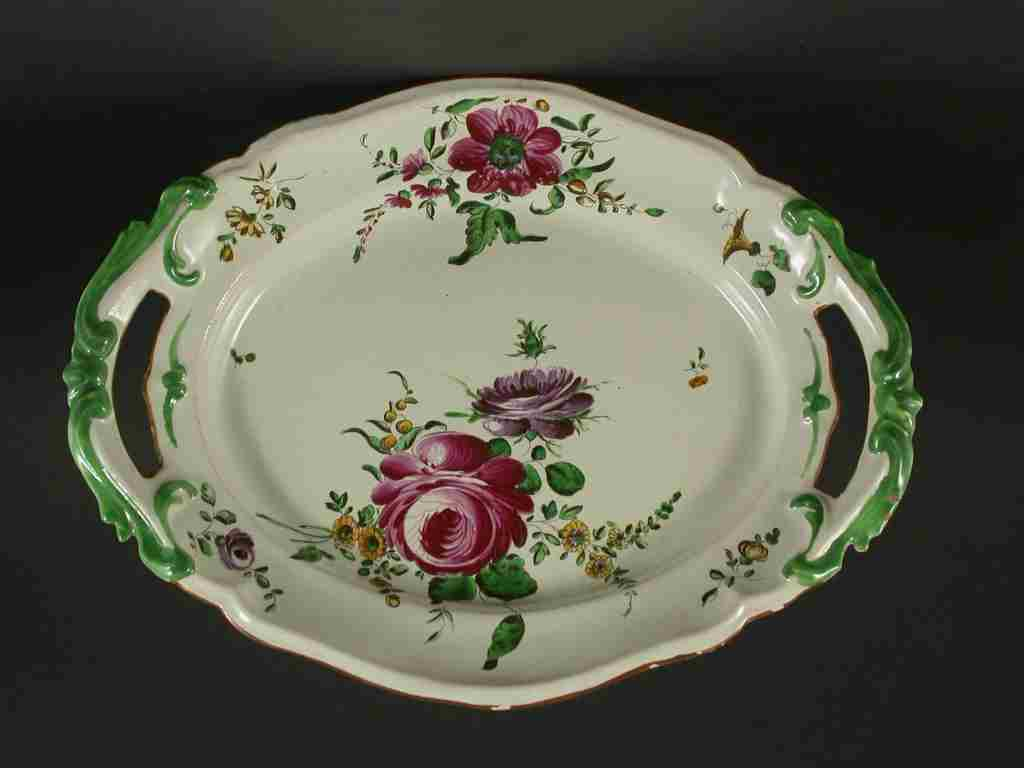
\includegraphics[scale=0.8]{Scacciani_Antonio-Vassoio-Rosa.jpg}
				\captionof{figure}{Scacciani Antonio - Vassoio - Rosa.}
			\end{minipage}
		\end{itemize}
	\end{frame}
	
	
	\begin{frame}{\numcirc{8} Mostrare il Mercato di Aureliano Milani.}
		\begin{itemize}
			\item Mostrare il dipinto ad olio Il Mercato di Aureliano Milani, che rappresenta una scena di vita quotidiana all'interno di un piccolo borgo abitato, in cui sono visibili diversi ceti sociali e i loro relativi mestieri.\par
		\end{itemize}
	\end{frame}
	
	\begin{frame}
		\bigskip
		\begin{minipage}{\linewidth}
			\centering
			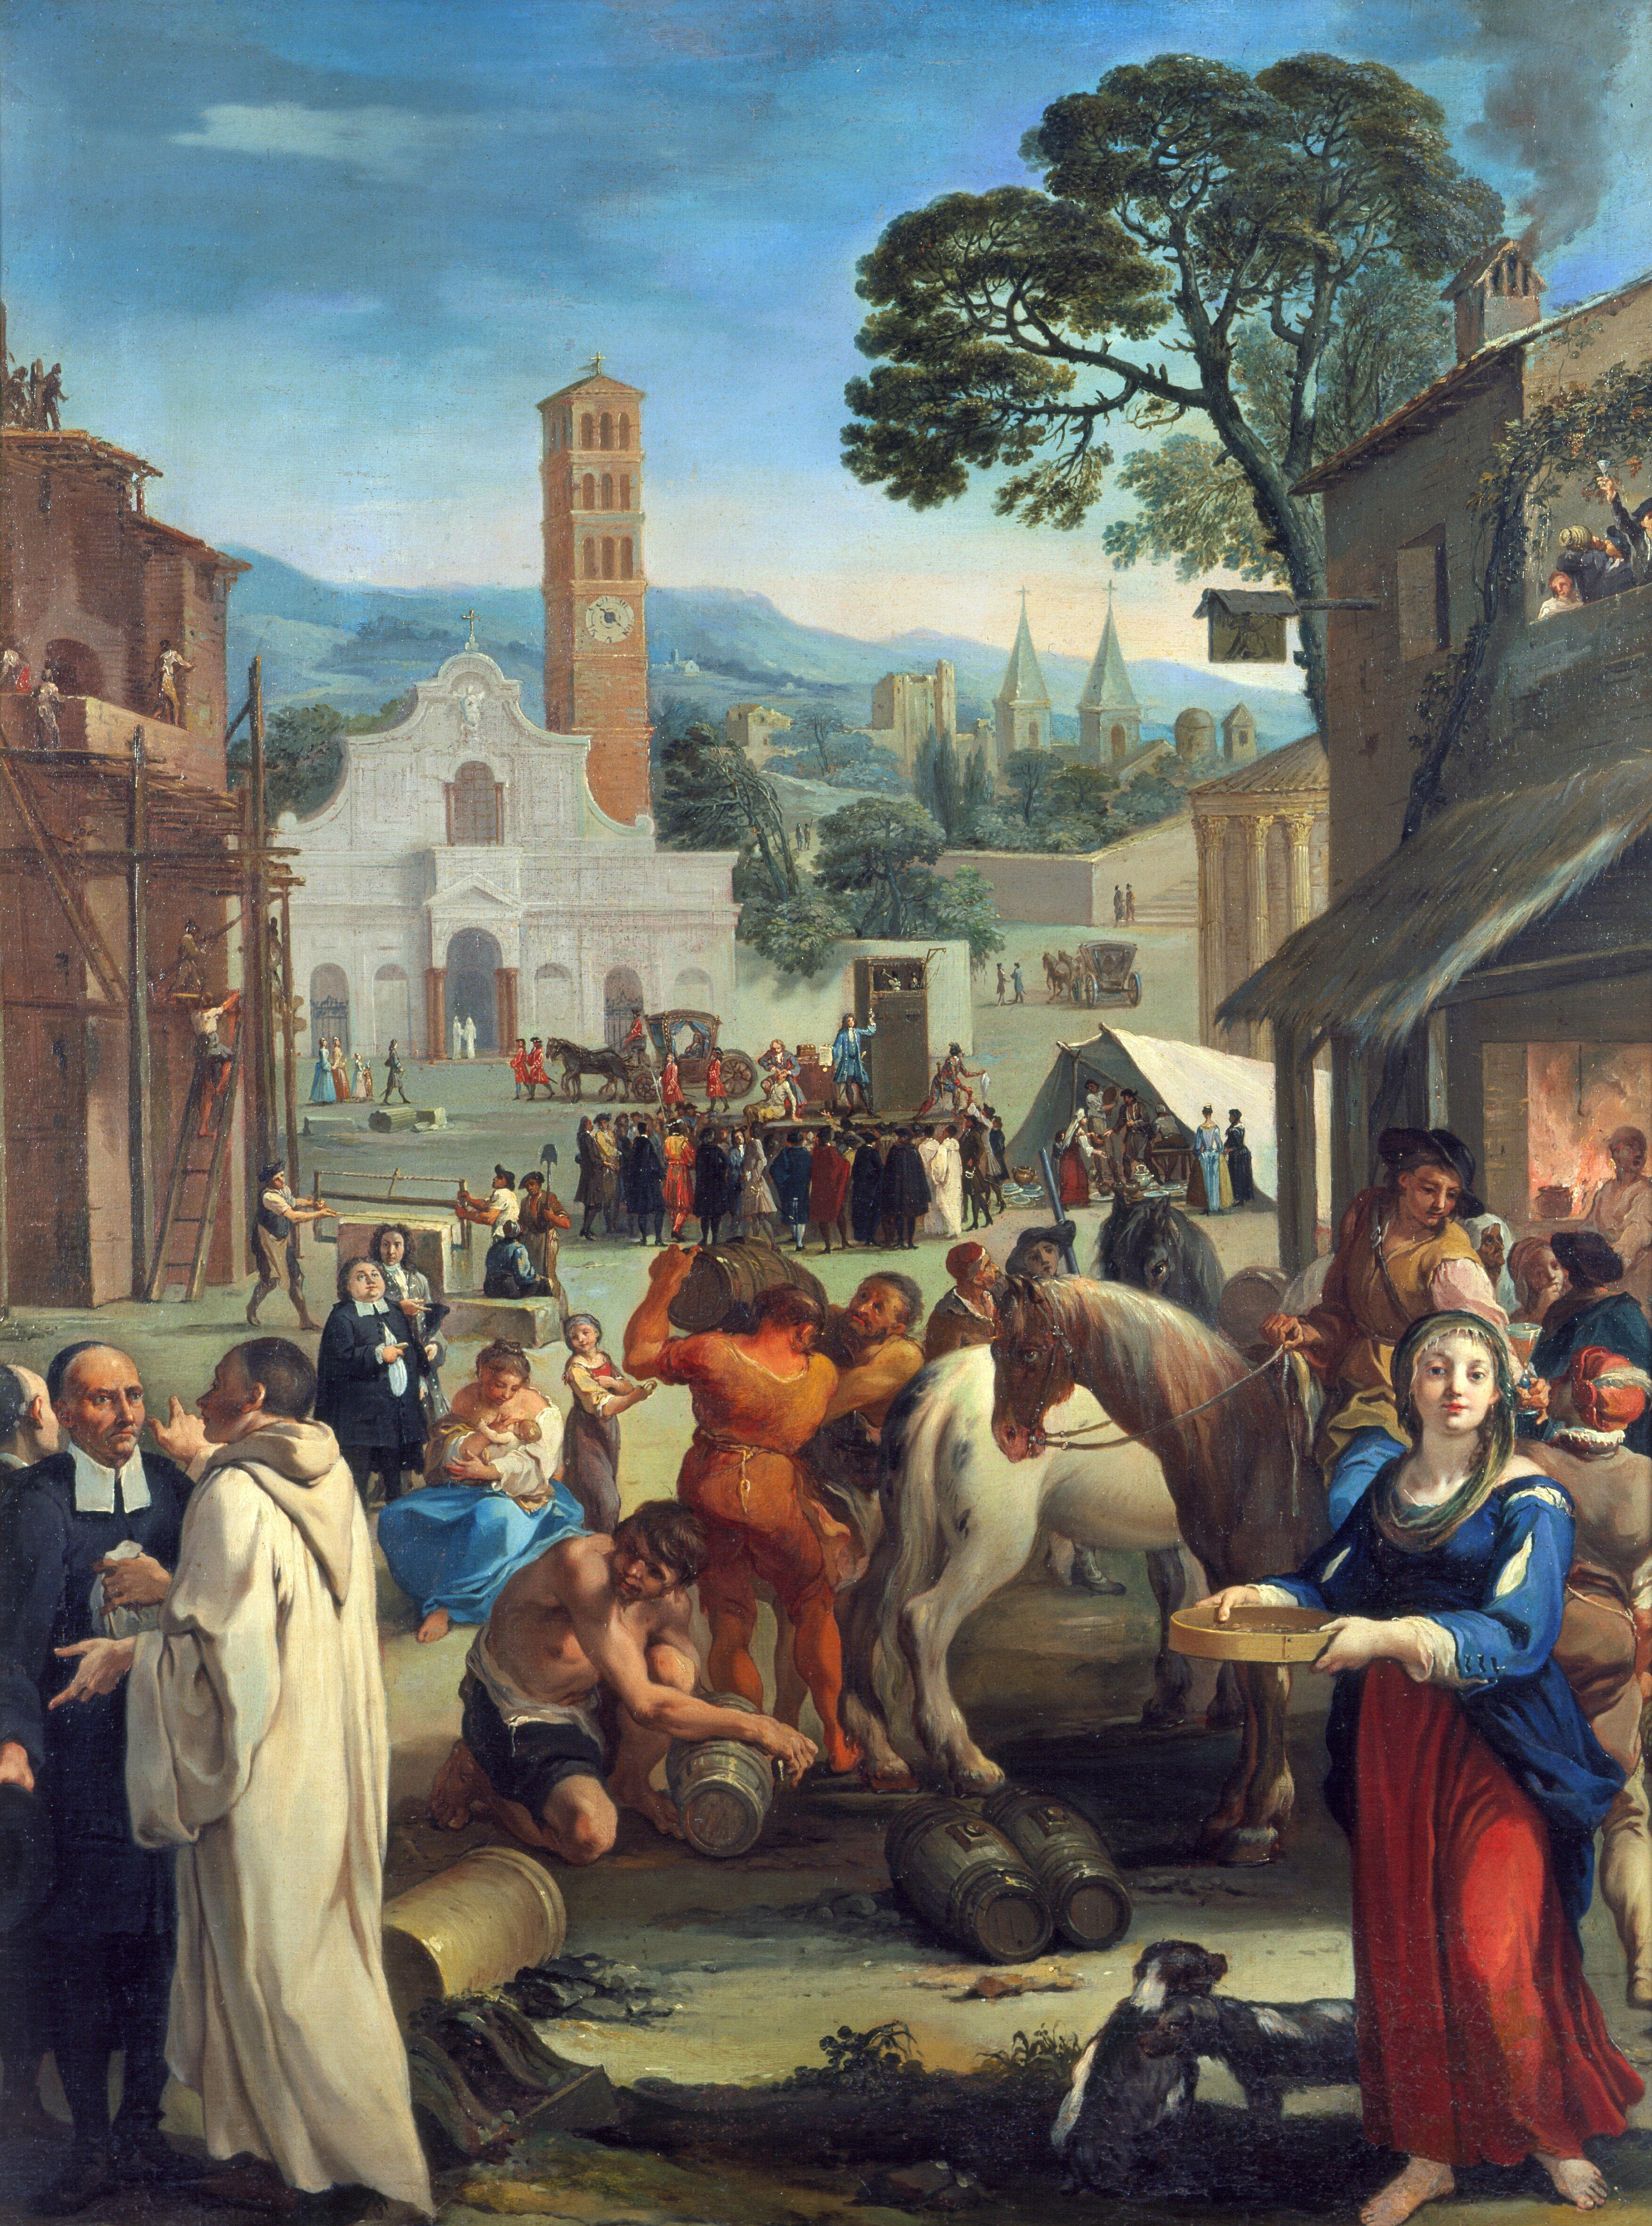
\includegraphics[scale=0.045]{Milani_Aureliano-Mercato.jpg}
			\captionof{figure}{Milani Aureliano - Mercato.}
		\end{minipage}
	\end{frame}

	\begin{frame}{\numcirc{9} Mostrare le Nature Morte.}
		\begin{itemize}
			\item Mostrare le \textbf{Nature Morte}, evidenziando la \textit{frutta} ed i \textit{calici in vetro}, mostrare il \textbf{Trompe l'oeil} con il \textit{Sonetto di Antonio Gianlisi Junior} e il \textbf{Trompe l'oeil} con la \textit{pipa} mettendo in risalto i cibi e gli oggetti di uso comune come la \textit{pipa} e i \textit{savoiardi} che alludono ai Savoia.\par
		\end{itemize}
	\end{frame}

	\begin{frame}
		\bigskip
		\begin{minipage}{\linewidth}
			\centering
			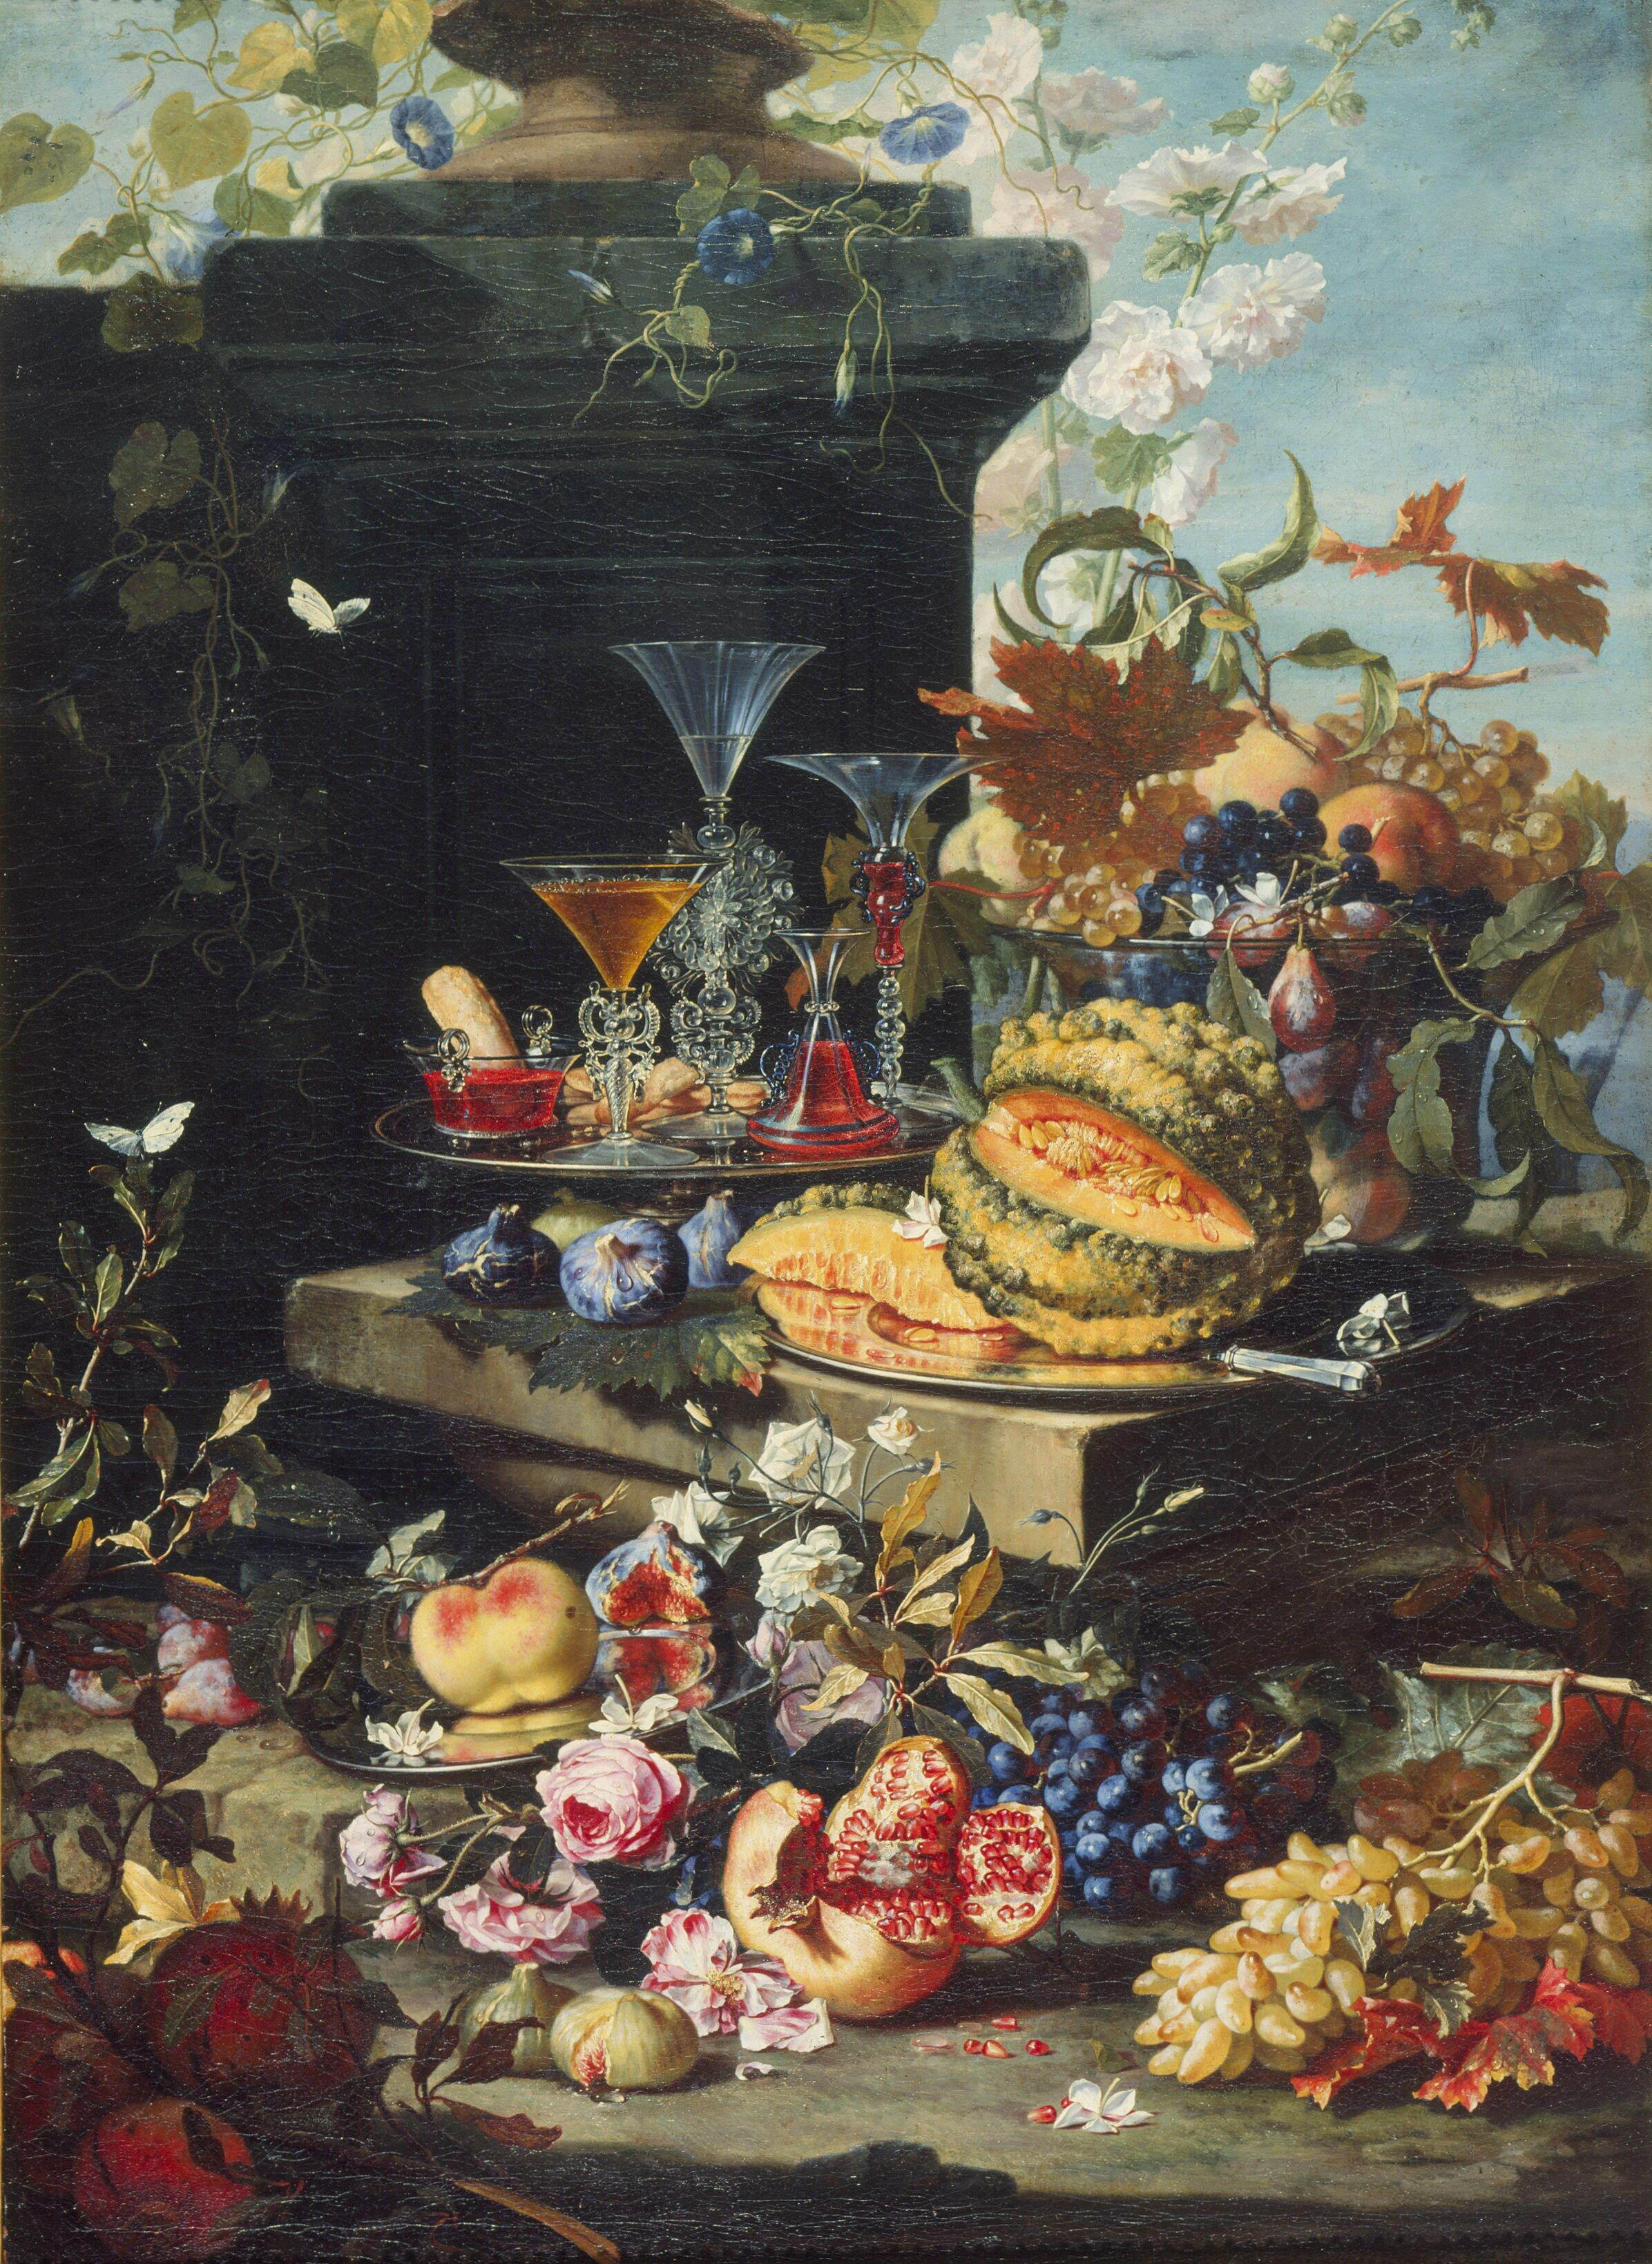
\includegraphics[scale= 0.06]{Berentz_Christian-Fiori_e_frutta_con_bicchieri_di_cristallo.jpg}
			\captionof{figure}{Berentz Christian - Fiori e frutta con bicchieri di cristallo.}
		\end{minipage}
	\end{frame}

	\begin{frame}
	\bigskip
	\begin{minipage}{\linewidth}
		\centering
		\begin{minipage}[t]{0.4\linewidth}
			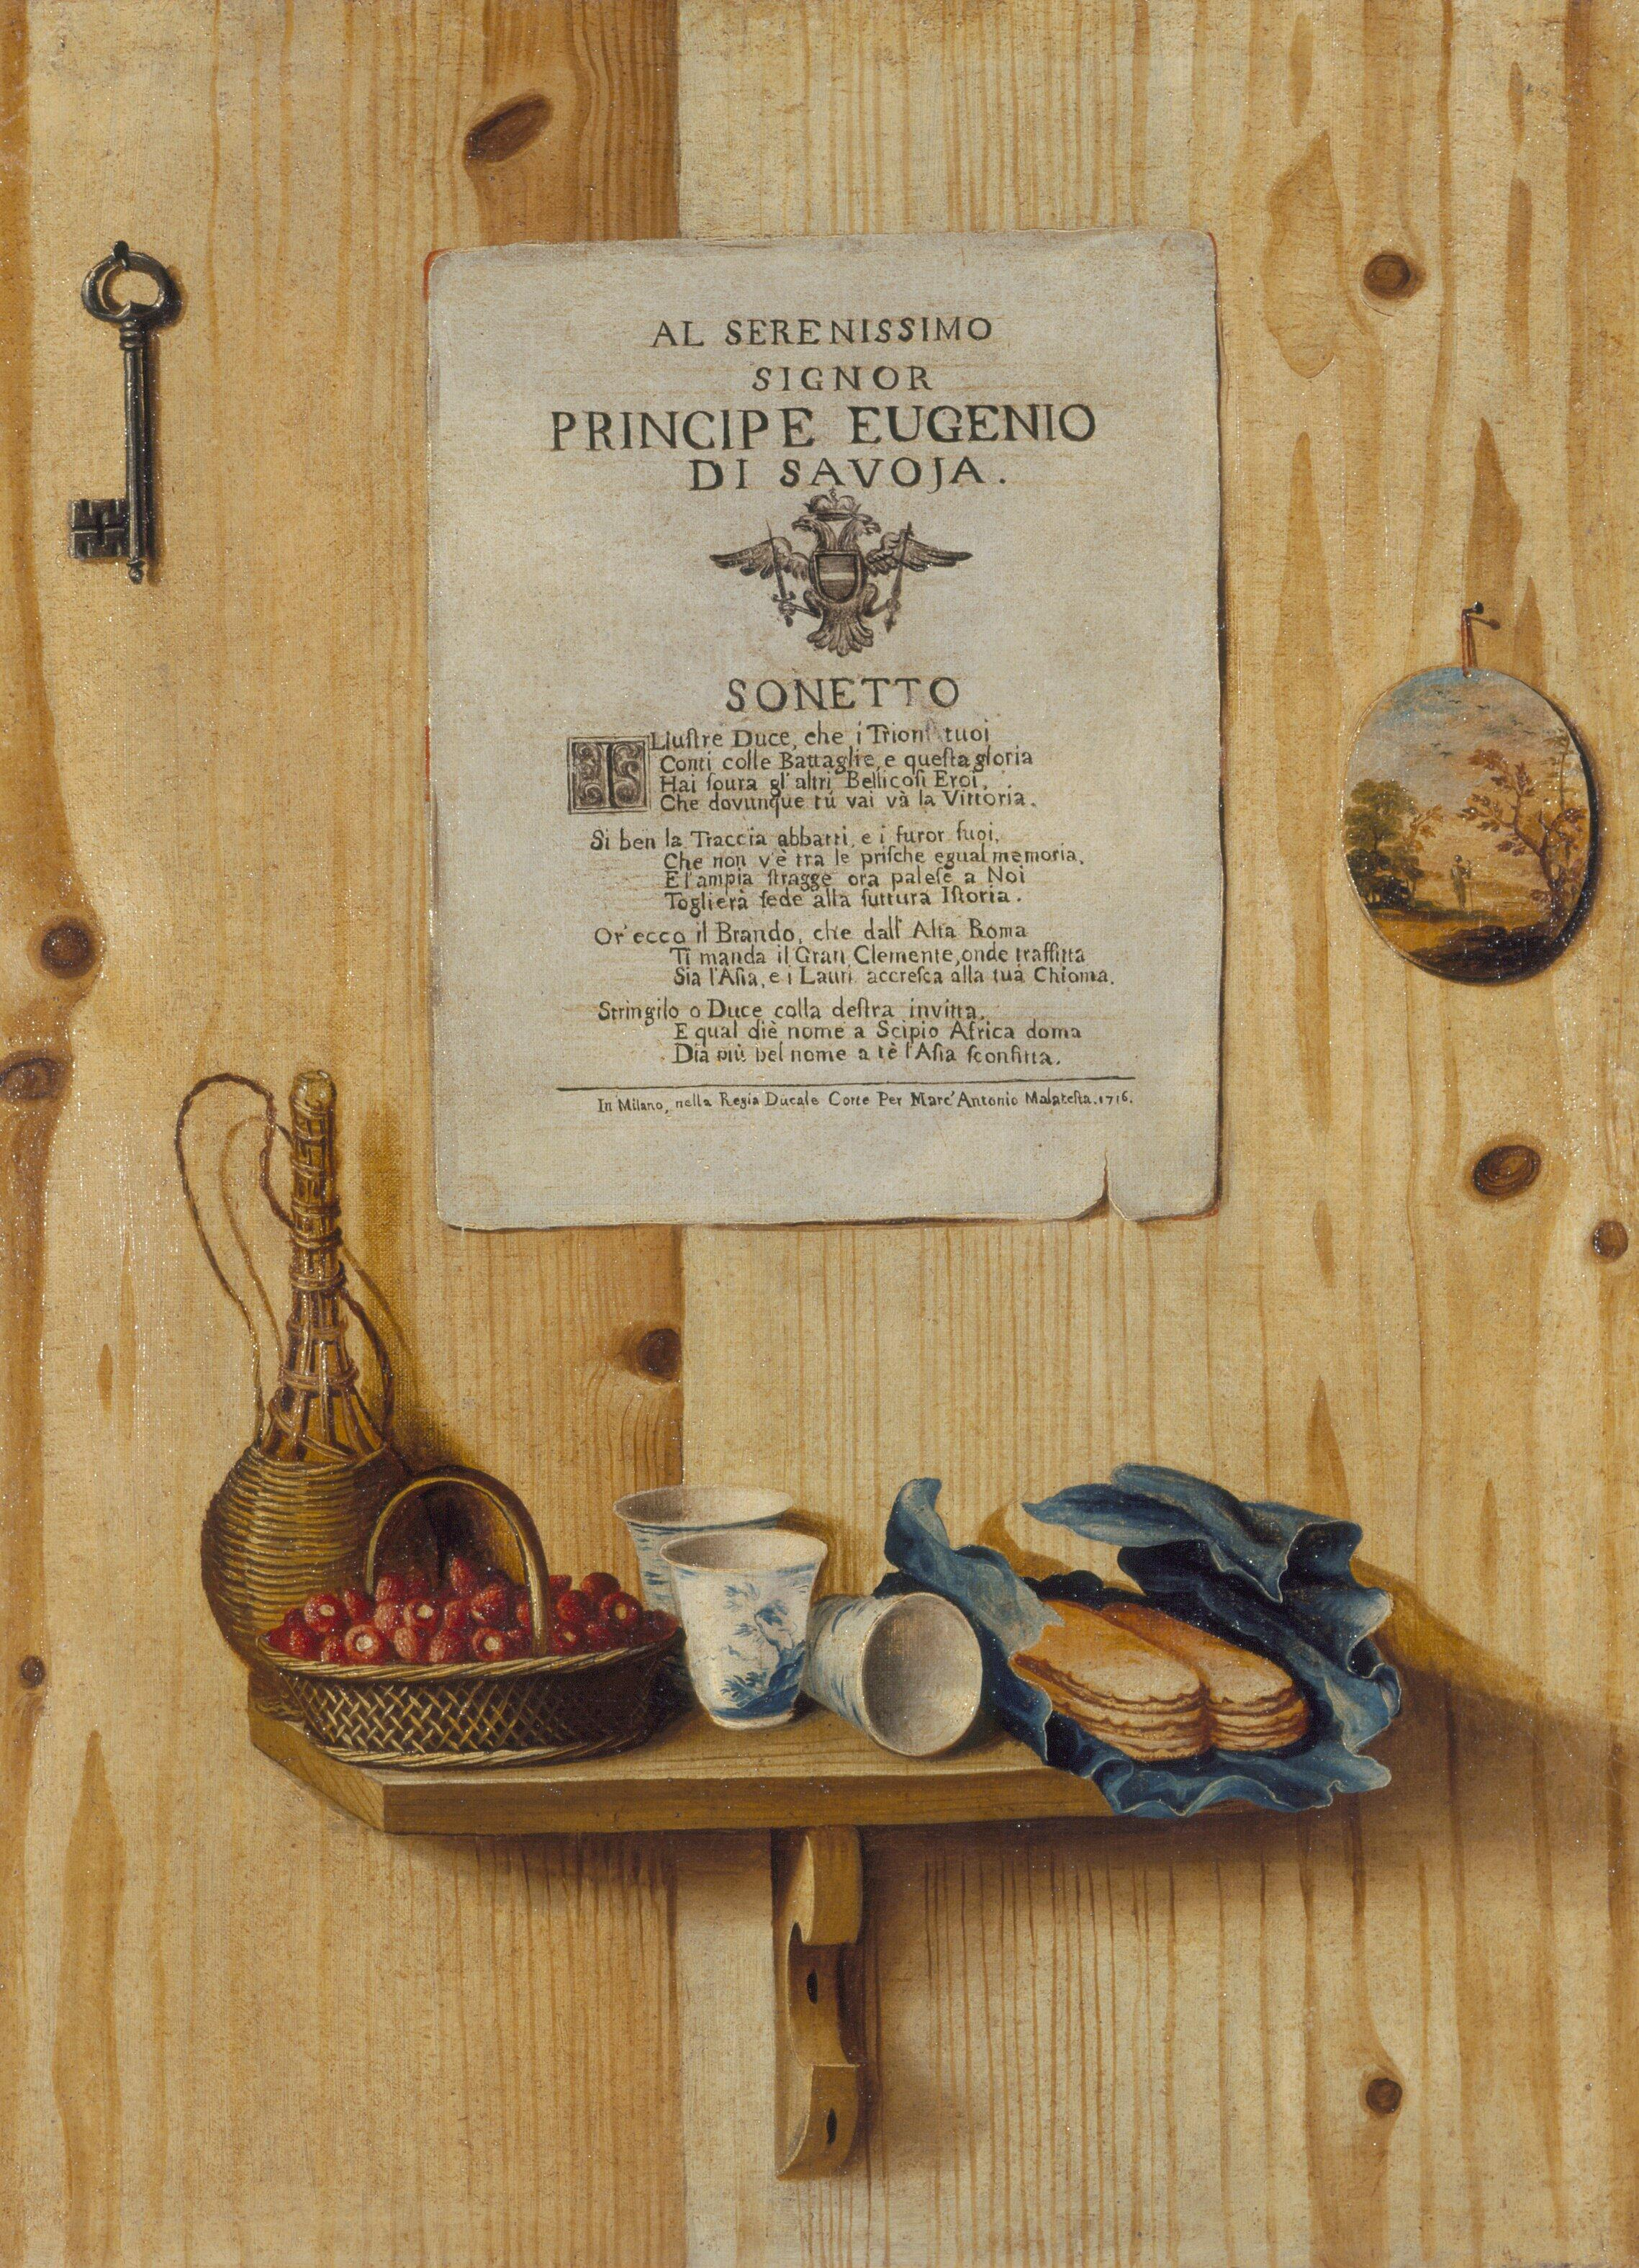
\includegraphics[scale=0.057]{Gianlisi_Antonio_Junior-Trompe_l_oeil_con_sonetto_in_onore_di_Eugenio_di_Savoia_e_mensola_con_oggetti.jpg}
			\captionof{figure}{Gianlisi Antonio Junior - Trompe l'oeil con sonetto in onore di Eugenio di Savoia e mensola con oggetti.}
		\end{minipage}
		\hfill
		\begin{minipage}[t]{0.4\linewidth}
			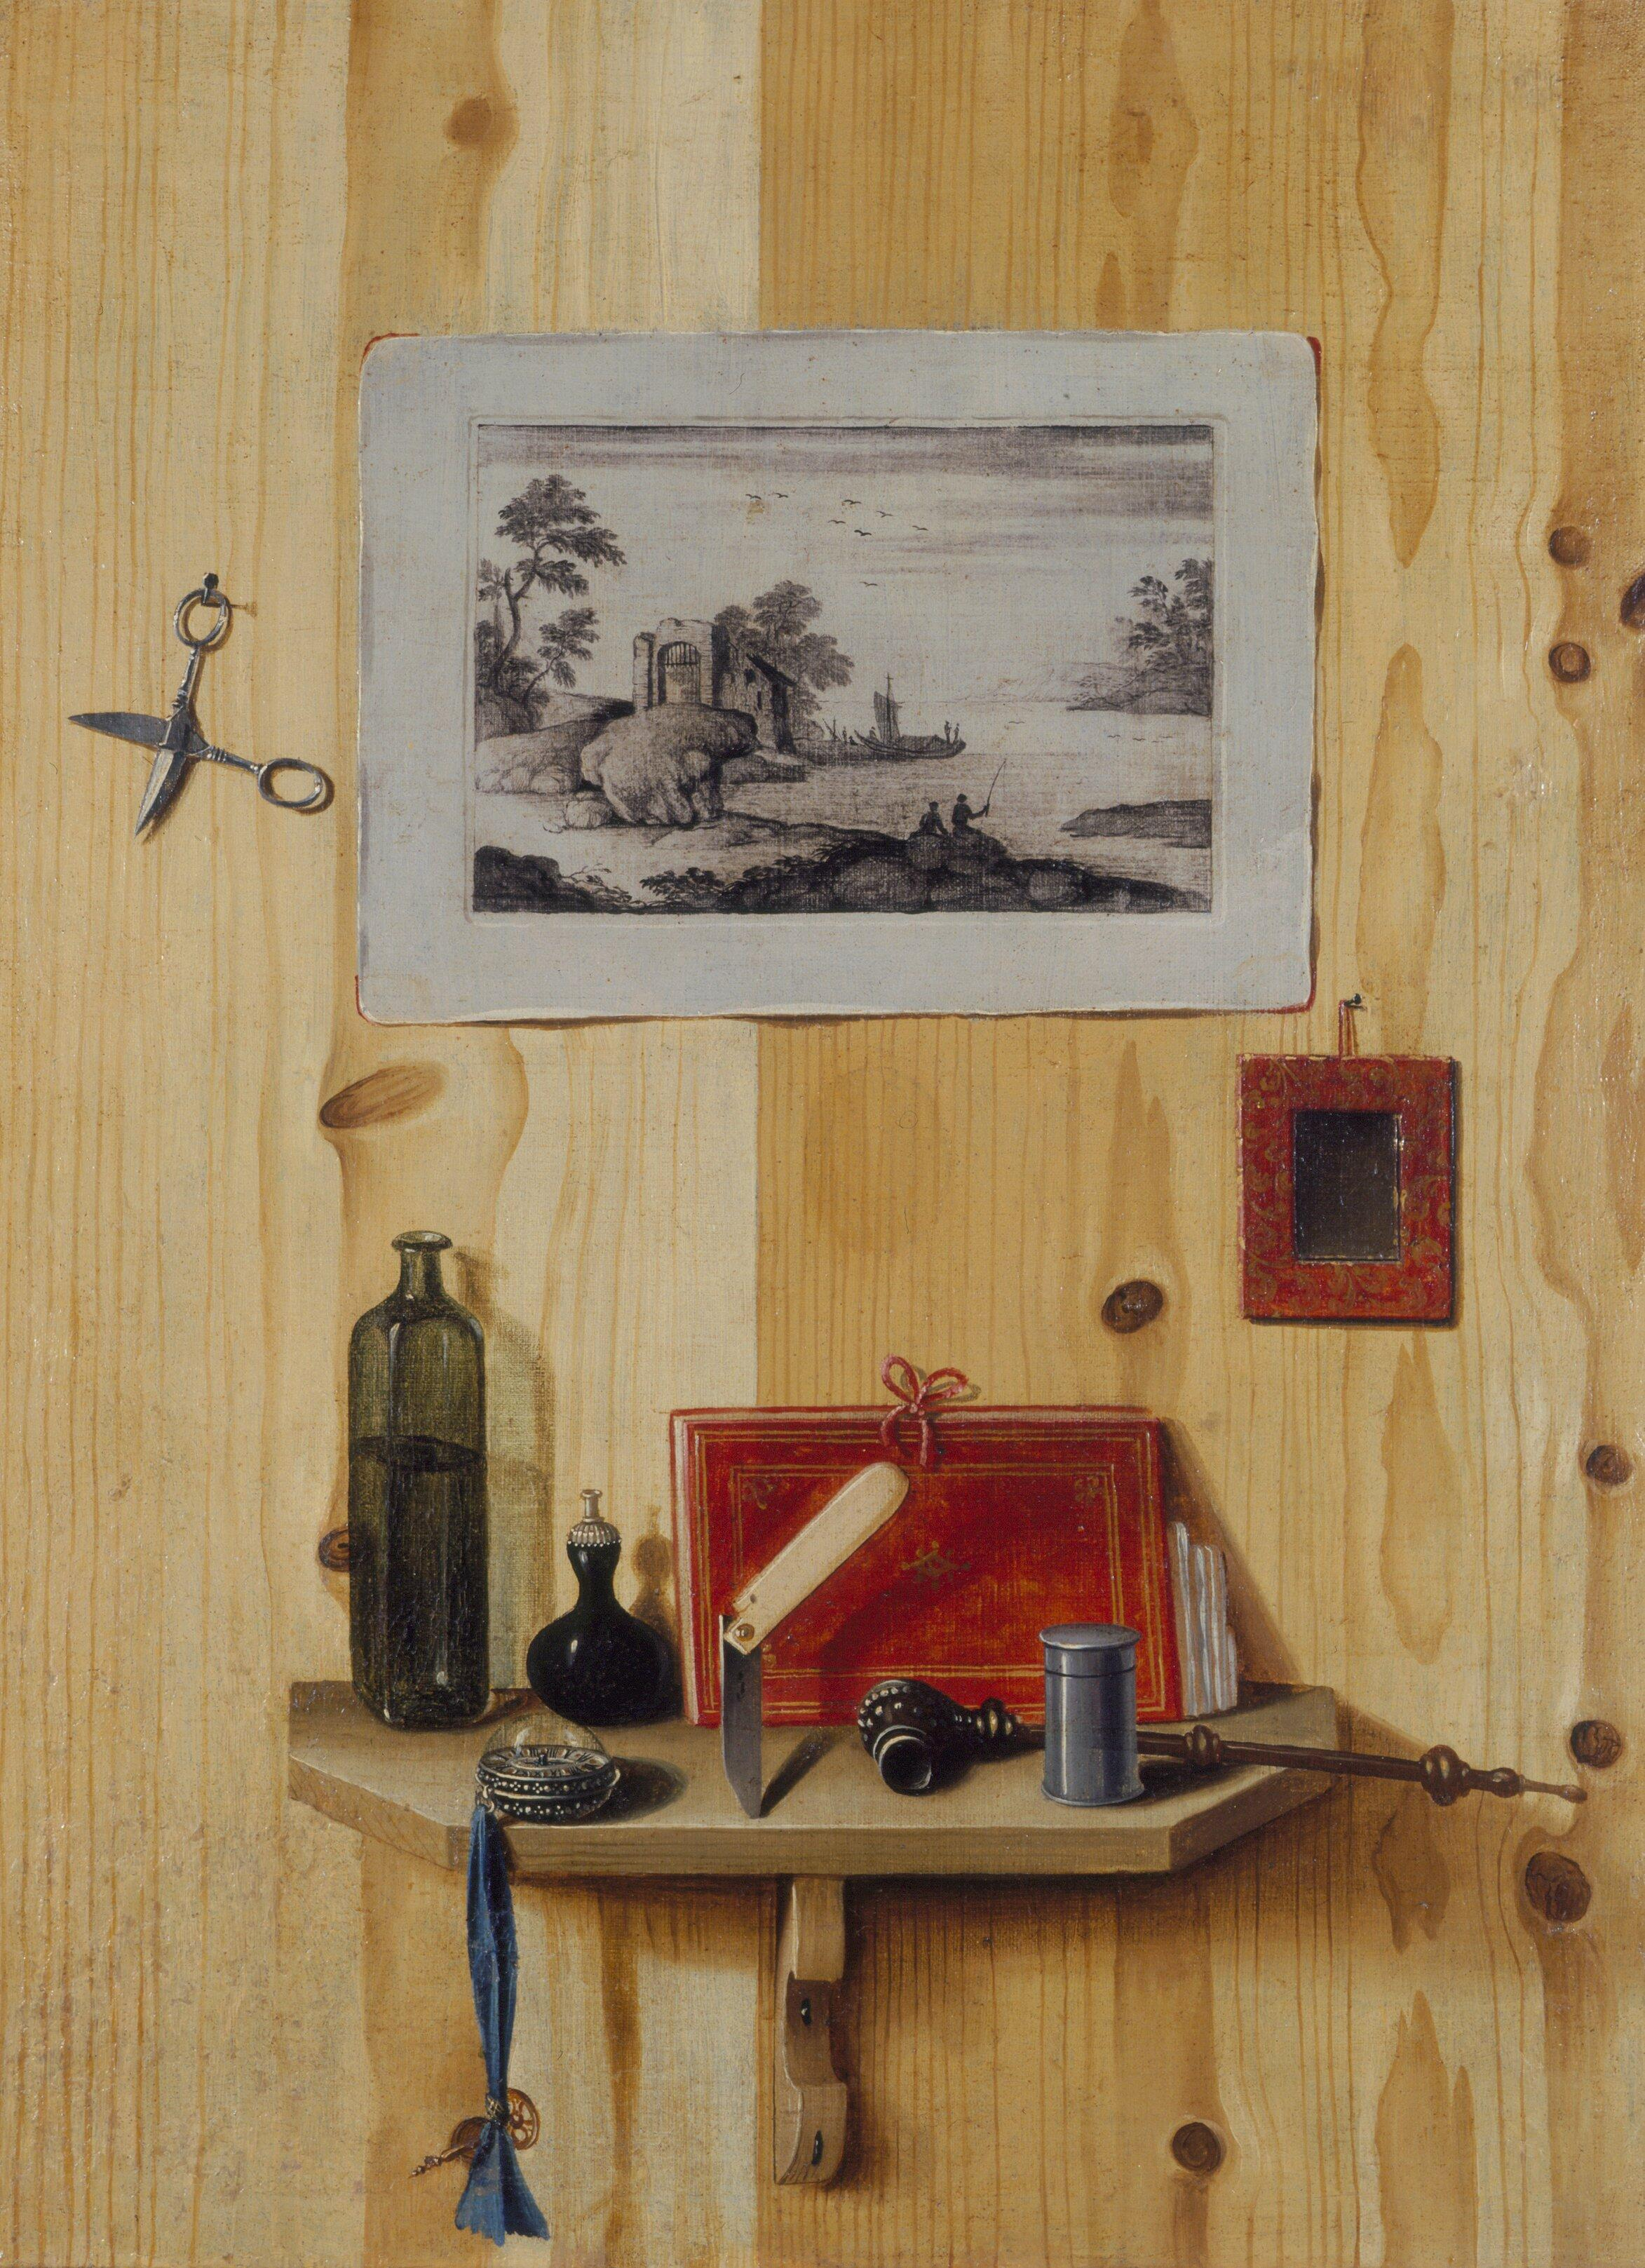
\includegraphics[scale=0.057]{Gianlisi_Antonio_Junior-Trompe_l_oeil_con_paesaggio_forbici_e_mensola_con_oggetti.jpg}
			\captionof{figure}{Gianlisi Antonio Junior - Trompe l'oeil con paesaggio forbici e mensola con oggetti.}
		\end{minipage}
	\end{minipage}
	\end{frame}
	
	\begin{frame}{\numcirc{10} Mostrare dipinti contenenti particolari che possono attirare l'attenzione dei bambini.}
		\begin{itemize}
			\item Mostrare dipinti contenenti particolari che possono attirare l'attenzione dei bambini, come per esempio \textit{le uova, i salami ed i limoni} nel dipinto \textbf{Dispensa con dolci, uova, salame, formaggi, ghiacciata e canestro di limoni} oppure il dettaglio del \textit{cinghiale} presente nella \textbf{Morte di Adone}.\par
		\end{itemize}
	\end{frame}
	
	\begin{frame}
		\bigskip
		\begin{minipage}{\linewidth}
			\centering
			\begin{minipage}[t]{0.4\linewidth}
			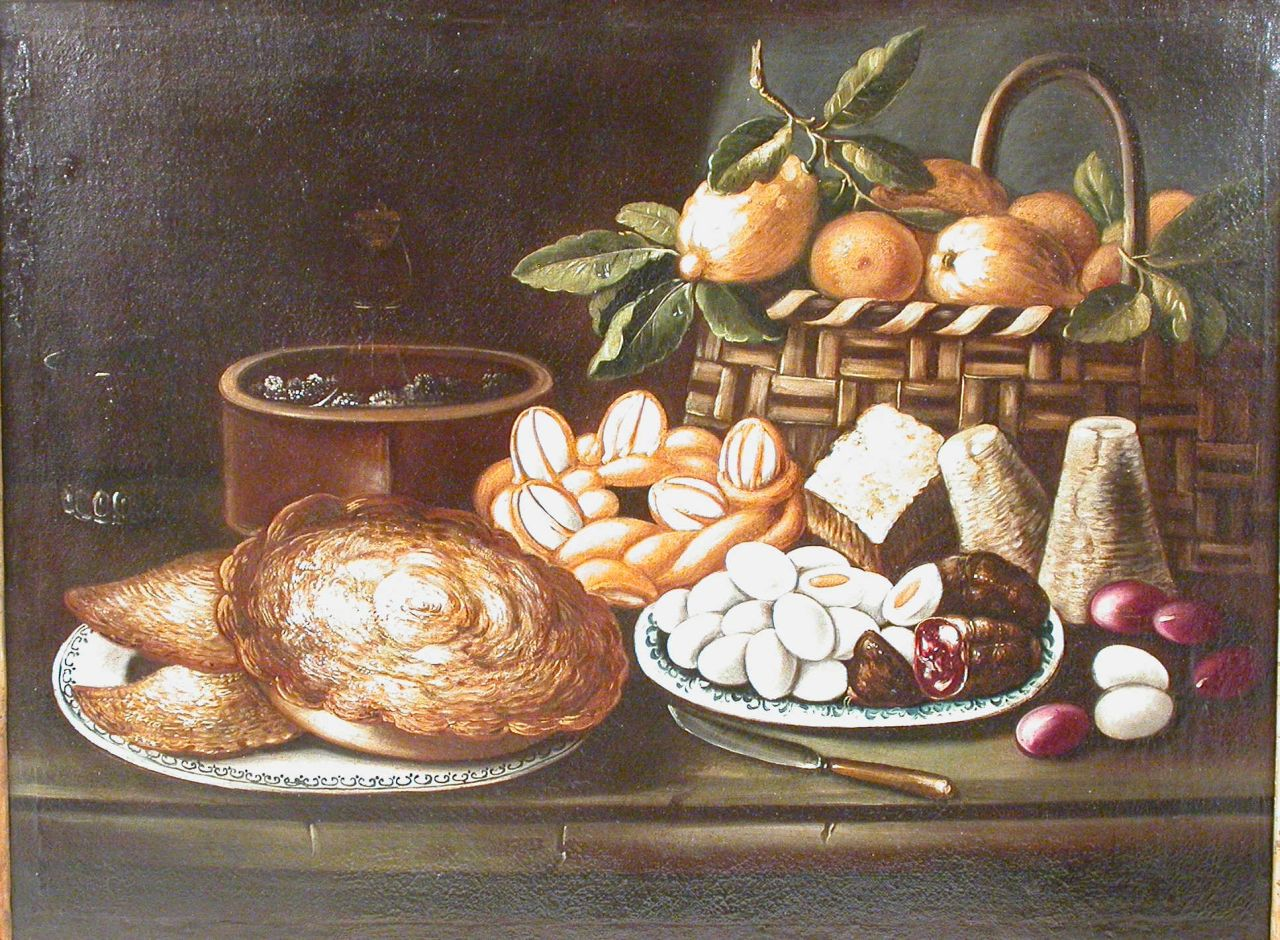
\includegraphics[scale=0.6]{Realfonzo_Tommaso-Natura_morta_con_dolci_frutta_uova_e_formaggi.jpg}
			\captionof{figure}{Realfonzo Tommaso - Natura morta con dolci frutta uova e formaggi.}
			\end{minipage}
			\hfill
			\begin{minipage}[t]{0.5\linewidth}
				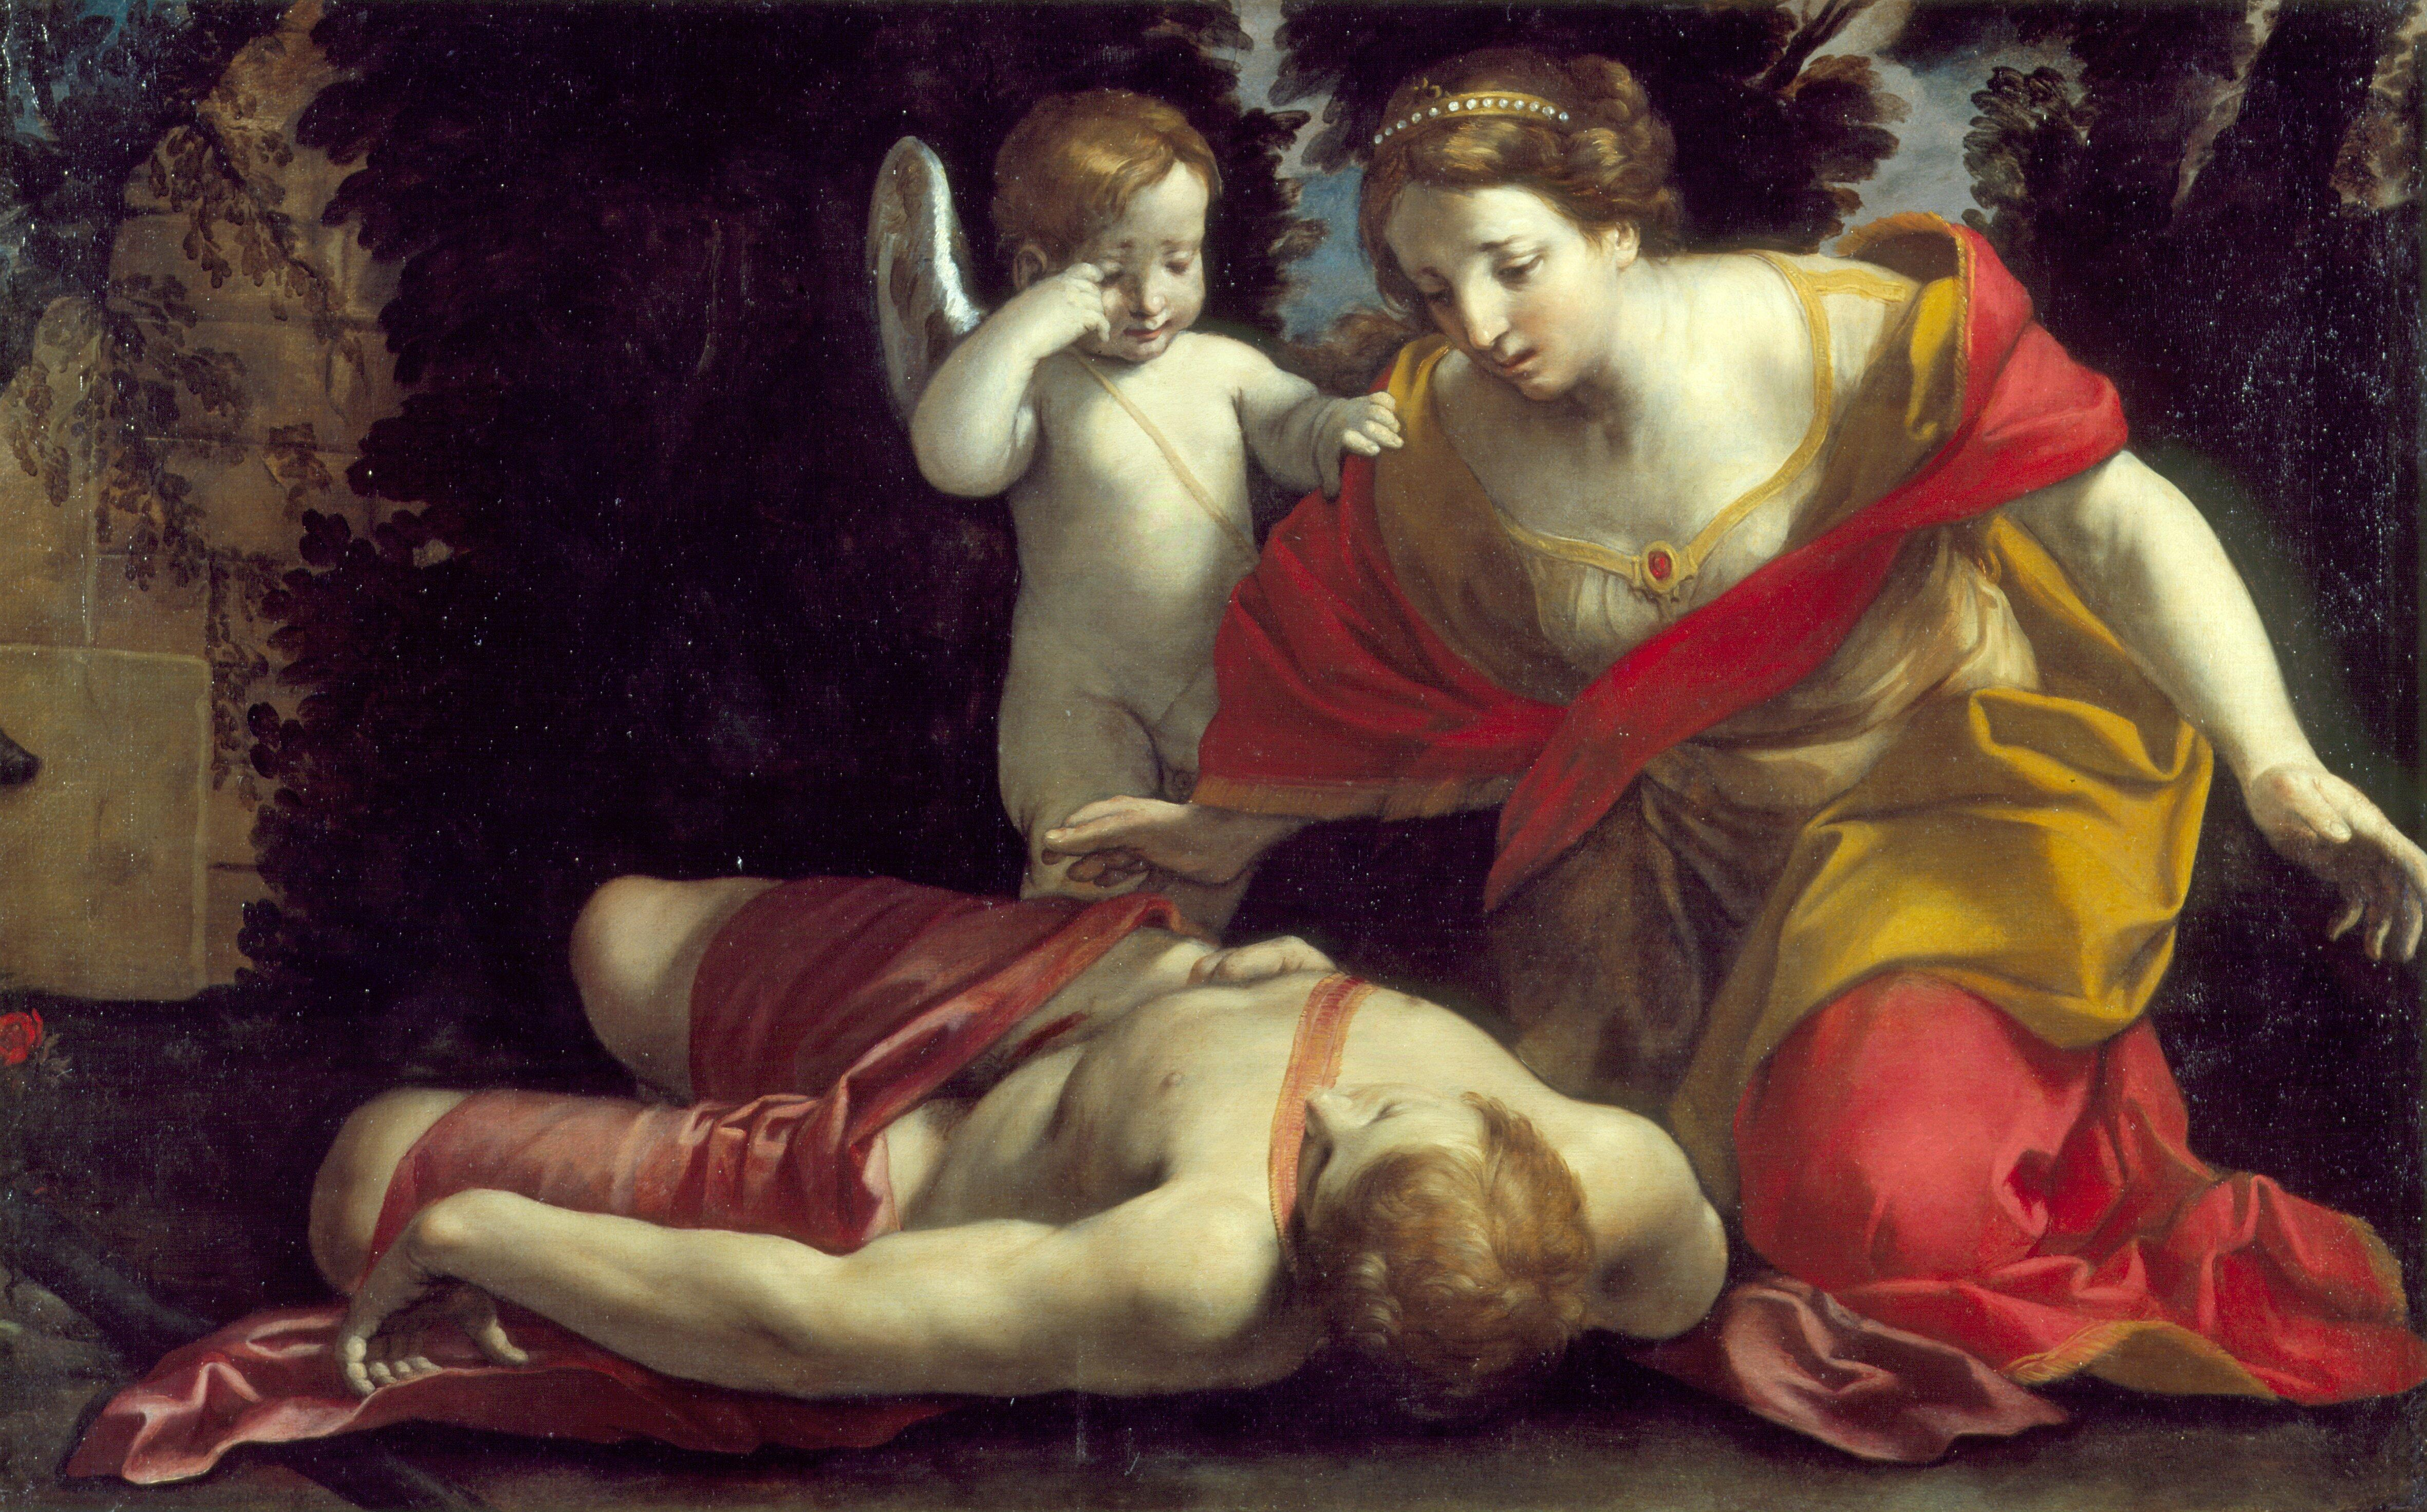
\includegraphics[scale=0.045]{Gessi_Giovan_Francesco-Morte_di_Adone.jpg}
				\captionof{figure}{Gessi Giovan Francesco - Morte di Adone.}
			\end{minipage}
		\end{minipage}
	\end{frame}
	
	\begin{frame}{\numcirc{11} Fare laboratori creativi con bambini.}
		\begin{itemize}
			\item \textbf{Per eventuali laboratori creativi con bambini gli può essere fornito un dettaglio dell'opera per poi far sì che vadano a ricercare essa all'interno del museo.}
		\end{itemize}
	\end{frame}
	
\end{document}